\chapter{Result and Discussion} \label{chp:result_and_discussion}

To assess the performance of the GBM, a case study will be conducted using the test dataset, which contains journey data for the entire year of 2021. The evaluation process consists of two main parts. The first part involves assessing the performance of the BBM, where the trained model will predict the ship's SOG. The output of BBM, which is the SOG, will be fed to the WBM to estimate the power and subsequently the bunker consumption. For further clarity regarding the methodology, the following steps are taken which are based on the proposed methodology shown in \Cref{fig:flowchart_BBM} and \Cref{fig:flowchart_WBM}. For generation of the BBM, the steps taken are:

\begin{enumerate}
    \setlength\itemsep{0em}
    \item Dataset is loaded.
    \item Identify and remove any anomalies.
    \item Remove static and unneeded features.
    \item Apply speed threshold of 5 knots.
    \item Highly correlated features are combined/removed based on physical and statistical reasoning.
    \item Impute missing values using {\tt KNNImputer}.
    \item Split the dataset into training and testing.
    \item Train the model using the whole dataset with default hyperparameter.
    \item Evaluate model performance using k-fold cross-validation.
    \item Tune the model until the best model is obtained.
    \item For the case study, the best models will be used to predict the SOG using the test dataset.
\end{enumerate}

Subsequently, for FOC calculation, the following steps are taken:

\begin{enumerate}
    \setlength\itemsep{0em}
    \item The test dataset is split into seasonal data. Summer-Fall season and Winter-Spring season corresponding to data for 6 months respectively.
    \item Impute missing values using {\tt KNNImputer}.
    \item SOG is converted to STW.
    \item Calculate calm water resistance $R_{CALM}$.
    \item Calculate added resistance due to wave $R_{AW}$.
    \item Calculate added resistance due to wind $R_{AA}$.
    \item Calculate total effective power $P_E$ using total resistance $R_{TOTAL}$.
    \item Calculate brake power $P_B$ from total efficiencies.
    \item Plot resulting regression line for Power-Speed curve from all models and actual case. 
    \item Calculate the FOC by considering the engine SFOC and operation time.
    \item Plot resulting regression line for FOC-Speed curve from all models and actual case.
    \item Evaluate the performance of the model generated from the regression lines.
\end{enumerate}

\section{Evaluation of BBM}\label{sec:BBM_tree_evaluate}

\subsection{Model Training and Selection of Optimal Parameter}\label{sec:hpo_select_train}

As noted in Section \ref{sec:BBM_modelling}, the training dataset encompasses 2871 data points. To refine the range of hyperparameter search for the tree-based model, MAE plots were generated against varying hyperparameter values, a technique outlined in \Cref{sec:hpo}. The hyperparameters are iteratively tuned until the optimal model is achieved. The outcome of this hyperparameter optimization process is presented in Table \ref{tbl:hpo_optimal}. The model training is conducted using an \textbf{AMD Ryzen 7 2700X, Eight-Core Processor} operating at 3.7 GHz, with 16384 MB of installed RAM.\\

\begin{table}[h!]
    \footnotesize
    \centering
    % \resizebox {\textwidth}{!}
    {\begin{tabular}{ p{0.1\linewidth} p{0.2\linewidth}  p{0.3\linewidth} p{0.25\linewidth}}
    \hline
    Model & Training time [s] &  Optimal Hyperparameter & Search Range \\
    \hline
    DTR & 0.044 & None \\
    $\text{DTR}_{OPT}$ & 0.021  & {\tt min\_samples\_split = 7} & [2,10] \\
    &&{\tt min\_samples\_leaf = 10} & [1,10] \\
    &&{\tt max\_features = 12} & [1,12]\\
    &&{\tt max\_depth = 8} & [1,10] and [None]\\
    RFR & 4.112 & None \\
    $\text{RFR}_{OPT}$ & 3.431  & {\tt min\_samples\_split = 2} & [2,10]\\
    &&{\tt min\_samples\_leaf = 1} & [1,10]\\
    &&{\tt max\_features = 10} & [6,12]\\
    &&{\tt max\_depth = 120} & [10,200] and [None]\\
    &&{\tt n\_estimators = 100} & [100,1000]\\
    ETR & 0.944 & None \\
    $\text{ETR}_{OPT}$ & 4.390  & {\tt min\_samples\_split = 9} & [1,10]\\
    &&{\tt min\_samples\_leaf = 1} & [1,10]\\
    &&{\tt max\_features = 12} [1,12]\\
    &&{\tt max\_depth = 120} & [10,200] and [None]\\
    &&{\tt n\_estimators = 800} & [100,1000]\\
    MLR & 0.004  & None\\
    \hline
    \end{tabular}}
\caption{Optimal hyperparameter with training time of each model}\label{tbl:hpo_optimal}
\end{table}

With the default hyperparameters, the RFR exhibits the lengthiest training duration, followed by the ETR and the DTR. This aligns with expectations, as RFR employs a greedy algorithm, seeking the optimal feature for node splitting, leading to increased training time. ETR, on the other hand, trains faster due to its random feature selection during node splitting. DTR displayed the shortest training time as it constructs only a single tree. However, in the case of the optimised model, ETR requires a lengthier training period compared to RFR. This discrepancy arises from the number of trees in the optimized model, controlled by the {\tt n\_estimator} parameter. The optimized ETR model has 800 trees, while RFR comprises 100 trees. Notably, the training time of the optimized DTR model is halved, as pruning the tree results in a simpler model requiring less time for training.\\

To further investigate the effect of hyperparameter optimisation, the learning curve of each tree-based model is plotted. For DTR, generated model with default parameter will result in a model that heavily overfits the training data, which is evident from the large gap between the training error and validation error which indicated a high variance as shown in \Cref{fig:learn_curve_TREE_MAE}. Regularisation i.e. parameter tuning of the DTR model helps balance between bias and variance by trading off bias for variance. This is observed from the substantial reduction in the gap between the training and validation error from \Cref{fig:learn_curve_TREE_MAE}. Additionally, the learning curve indicates that the model performance can be improved by increasing the amount of data points as the MAE continue to decrease with increasing amount of data points.\\

The process of hyperparameter tuning for the Random Forest Regressor (RFR) model did not show any significant improvement in model performance. This outcome aligns with the findings of  \bcitet{Kuhn.2013} and \bcitet{Hastie.2009} which was discussed in \Cref{sec:rf_theo}. The model starts to plateau at approximately 1000 data points. Furthermore, there is a noticeable variance in the RFR model, which indicates that the model will have a slight tendency to overfit. On the other hand, hyperparameter tuning contributes to variance reduction in the ETR model. However, its impact on overall model performance remains limited. The ETR model reaches a performance plateau beyond 1000 data points, indicating that augmenting the dataset with additional points is unlikely to yield substantial improvements in model effectiveness.\\


\begin{figure}
    \centering
    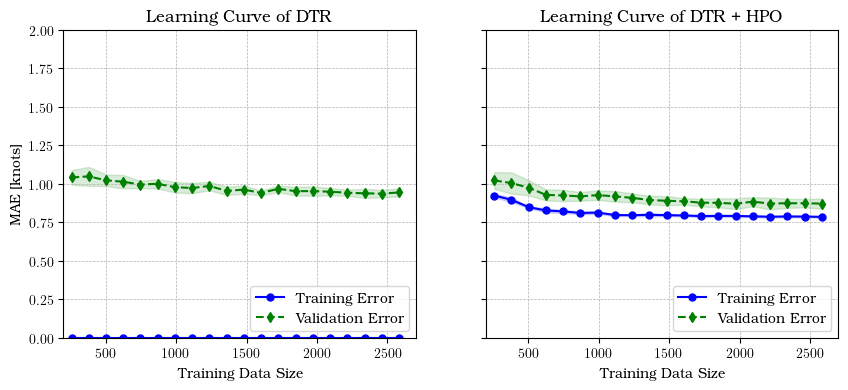
\includegraphics[width=.95\textwidth]{02_figures/learning_curve_dtr_mae.png}\\
    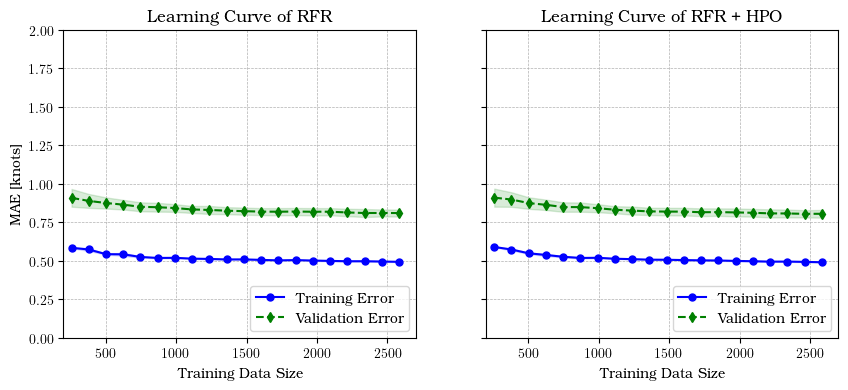
\includegraphics[width=.95\textwidth]{02_figures/learning_curve_rfr_mae.png}\\
    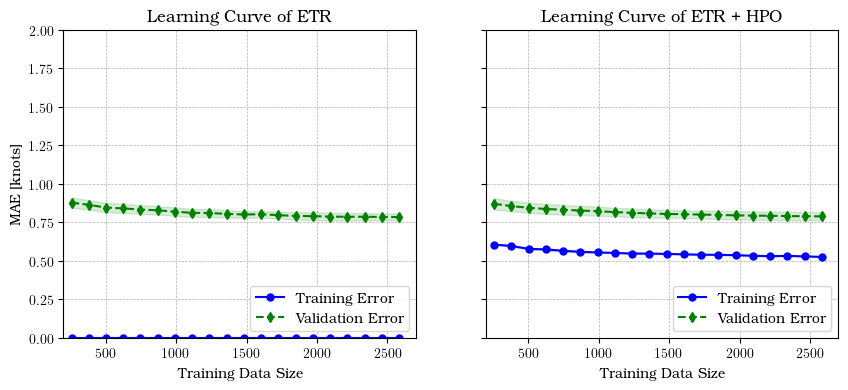
\includegraphics[width=.95\textwidth]{02_figures/learning_curve_etr_mae.png}
    \caption{Learning curve of various tree-based models}
    \label{fig:learn_curve_TREE_MAE}
\end{figure}

% \begin{figure}[h]
%     \centering
%         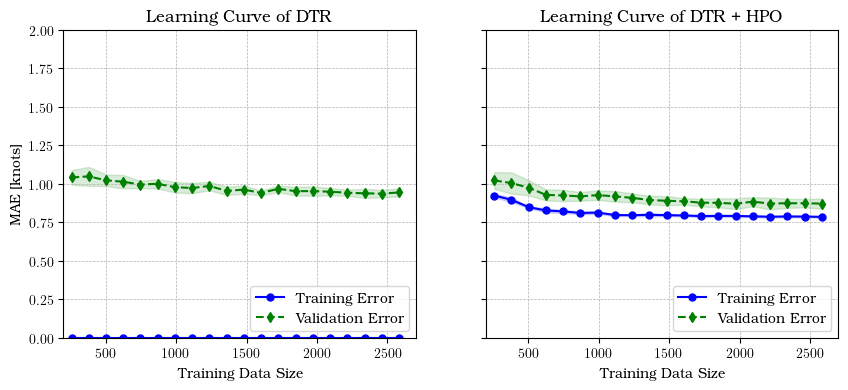
\includegraphics[width=.95\textwidth]{02_figures/learning_curve_dtr_mae.png}
%         \caption{Learning curve of DTR}
%         \label{fig:learn_curve_DTR_MAE}
% \end{figure}

% \begin{figure}[h]
%     \centering
%         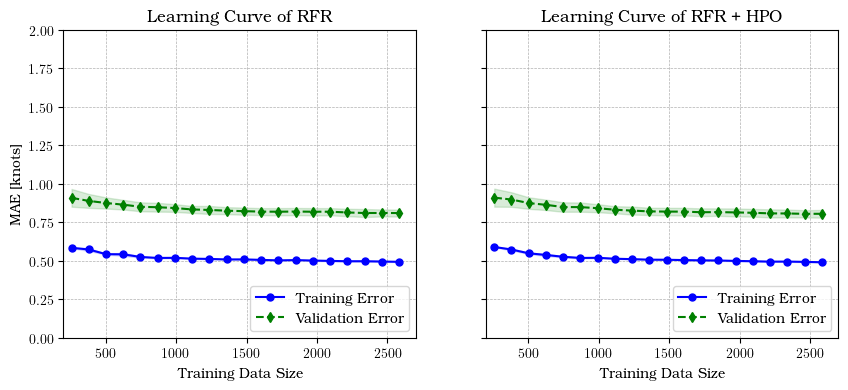
\includegraphics[width=.95\textwidth]{02_figures/learning_curve_rfr_mae.png}
%         \caption{Learning curve of RFR}
%         \label{fig:learn_curve_RFR_MAE}
% \end{figure}

% \begin{figure}[h]
%     \centering
%         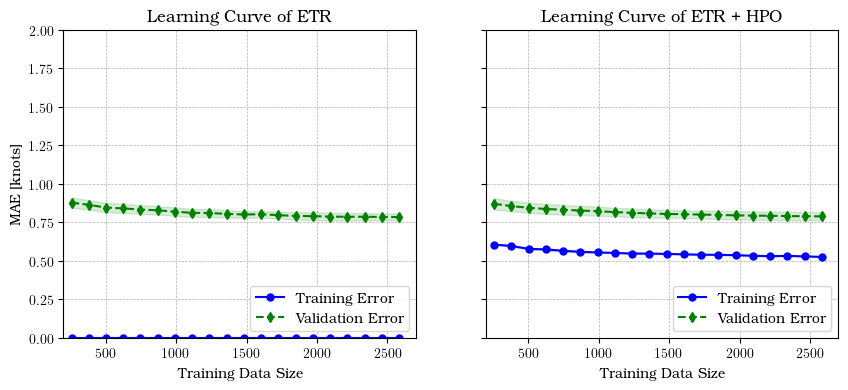
\includegraphics[width=.95\textwidth]{02_figures/learning_curve_etr_mae.png}
%         \caption{Learning curve of ETR}
%         \label{fig:learn_curve_ETR_MAE}
% \end{figure}

\pagebreak

\subsection{Analysis of trained model}\label{sec:BBM_model_eval}

\subsubsection{Feature Importance}\label{sec:feature_importance_bbm}

As discussed in \Cref{sec:rf_theo}, tree-based models inherently possess the ability to quantify the influence of each feature during the splitting process. This is performed using {\tt feature\_importances\_} feature in \scikit/ \bcitep{Kuhn.2013}. According to documentation by \bcitet{FabianPedregosa.2011}, this attribute is computed as the mean and standard deviation of the accumulated reduction in impurity within each tree, which is essentially the total reduction in the criterion achieved by a specific feature. Alternatively, it can be interpreted as a measure of how extensively a feature is employed in each tree.\\

\begin{table}[h]
    \scriptsize
    \centering
    \resizebox {\textwidth}{!}
    {\begin{tabular}{ p{0.15\linewidth} c| p{0.15\linewidth} c| p{0.15\linewidth} c}
    \hline
    $\text{DTR}_{OPT}$ & & $\text{RFR}_{OPT}$ & & $\text{ETR}_{OPT}$\\
    \hline
    Feature & Importance & Feature & Importance & Feature & Importance\\
    \hline
    {\tt heading} & 0.6563 & {\tt heading} & 0.4927 & {\tt cog} & 0.6410 \\
    {\tt cog} & 0.3183 & {\tt cog} & 0.4183 & {\tt heading} & 0.2707 \\
    {\tt draught} & 0.0105 & {\tt draught} & 0.0210 & {\tt truecurrentdir} & 0.0200\\
    {\tt truewinddir} & 0.0047 & {\tt curspeed} & 0.0104 & {\tt draught} & 0.0144 \\
    {\tt oceantemperature} & 0.0029 & {\tt waveperiod} & 0.0093& {\tt windwaveswellheight} & 0.0112\\
    {\tt surftemp} & 0.0025&{\tt truecurrentdir} & 0.0092 & {\tt curspeed} & 0.0110\\
    {\tt waveperiod} & 0.0019 & {\tt windwaveswellheight} & 0.0084& {\tt waveperiod} & 0.0095 \\
    {\tt truecurrentdir} & 0.0010 & {\tt surftemp} & 0.0075& {\tt windspeed} & 0.0053\\
    {\tt windwaveswellheight} & 0.0008 & {\tt truewinddir} & 0.0075& {\tt surftemp} & 0.0046 \\
    {\tt curspeed} & 0.0004 & {\tt truewavedir} & 0.0058& {\tt truewavedir} & 0.0045 \\
    {\tt windspeed} & 0.0004 & {\tt oceantemperature} & 0.0057& {\tt oceantemperature} & 0.0044\\
    {\tt truwavedir} & 0.0001 & {\tt windspeed} & 0.0056& {\tt truewinddir} & 0.0033\\
    \end{tabular}}
\caption{Feature importance of different models}\label{tbl:feature_importances}
\end{table}

The feature importances for all tree-based models shown in \Cref{tbl:feature_importances} indicated that the structure of the model is significantly influenced by the features {\tt heading} and {\tt cog}. This observation suggests that the models rely considerably on ship movement direction, represented by heading and COG, to predict the SOG at a given location. However, from a physical perspective, it will be more insightful to consider the ship state and weather conditions that affect the prediction of the SOG.\\

\begin{figure}
    \centering
    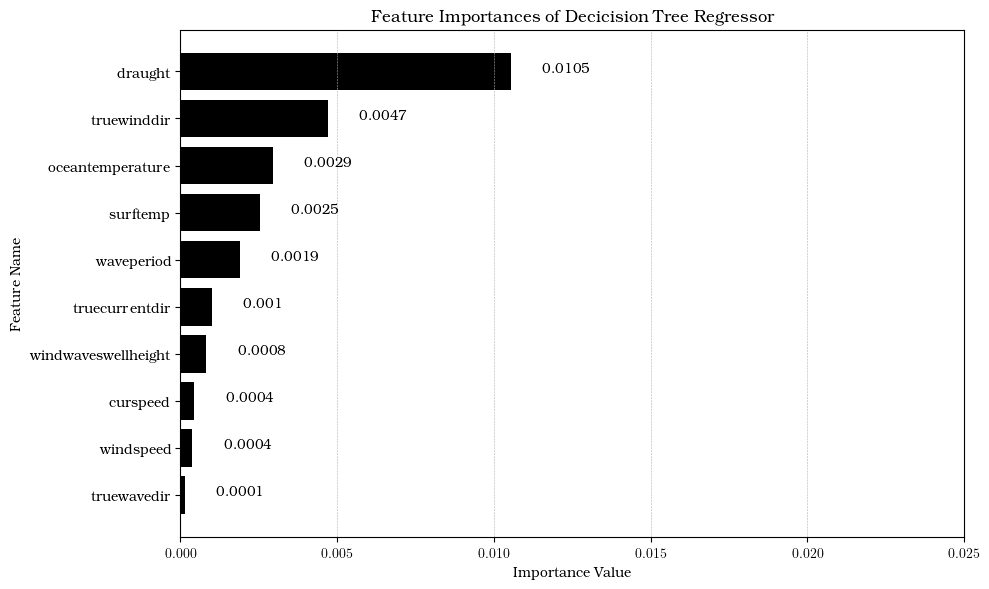
\includegraphics[width=.82\textwidth]{02_figures/dtr_ftr_importance_nodir.png}\\
    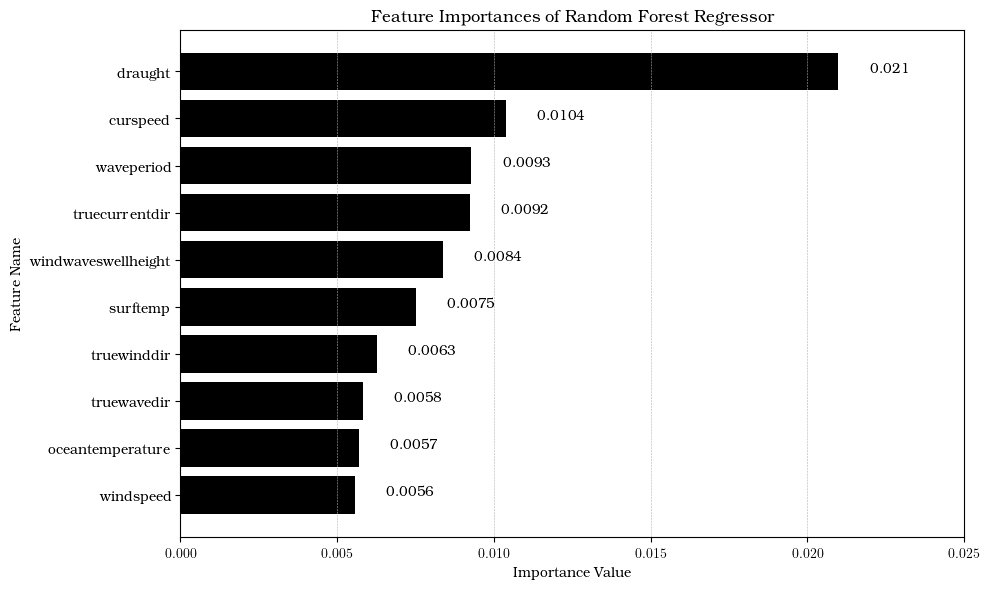
\includegraphics[width=.82\textwidth]{02_figures/rfr_ftr_importance_nodir.png}\\
    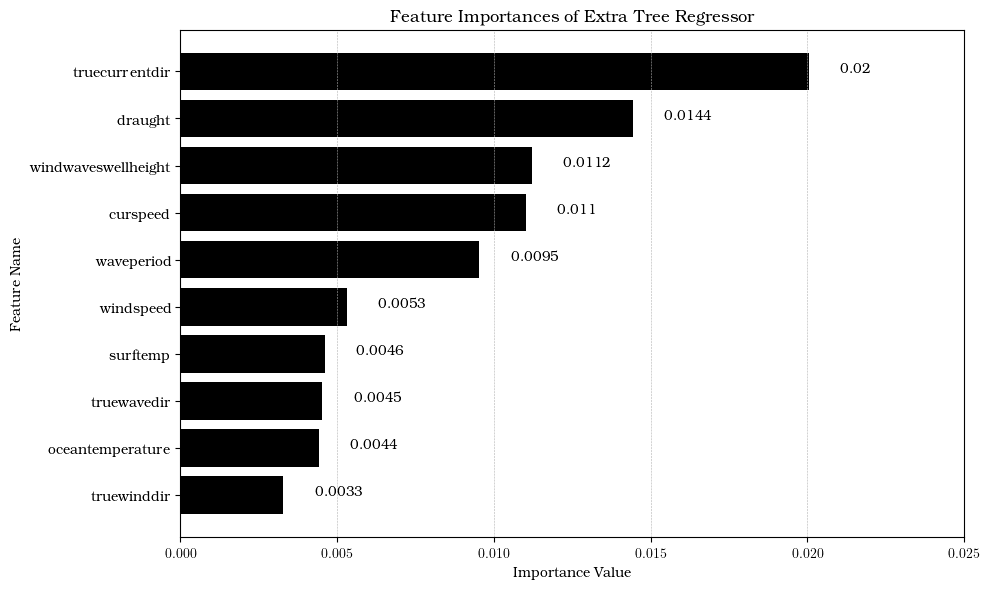
\includegraphics[width=.82\textwidth]{02_figures/etr_ftr_importance_nodir.png}
    \caption{Feature importance of different tree-based models}
    \label{fig:ftr_impo_overall_tree}
\end{figure}

% \begin{figure}[h]
%     \centering
%         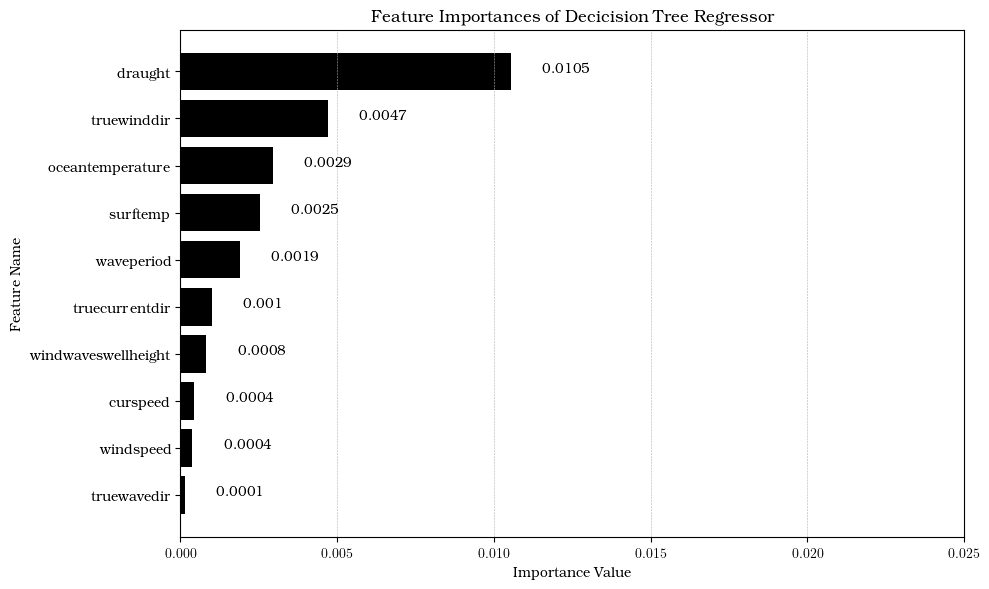
\includegraphics[width=.9\textwidth]{02_figures/dtr_ftr_importance_nodir.png}
%         \caption{Feature importance of DTR}
%         \label{fig:ftr_impo_dtr}
% \end{figure}

% \begin{figure}[h]
%     \centering
%         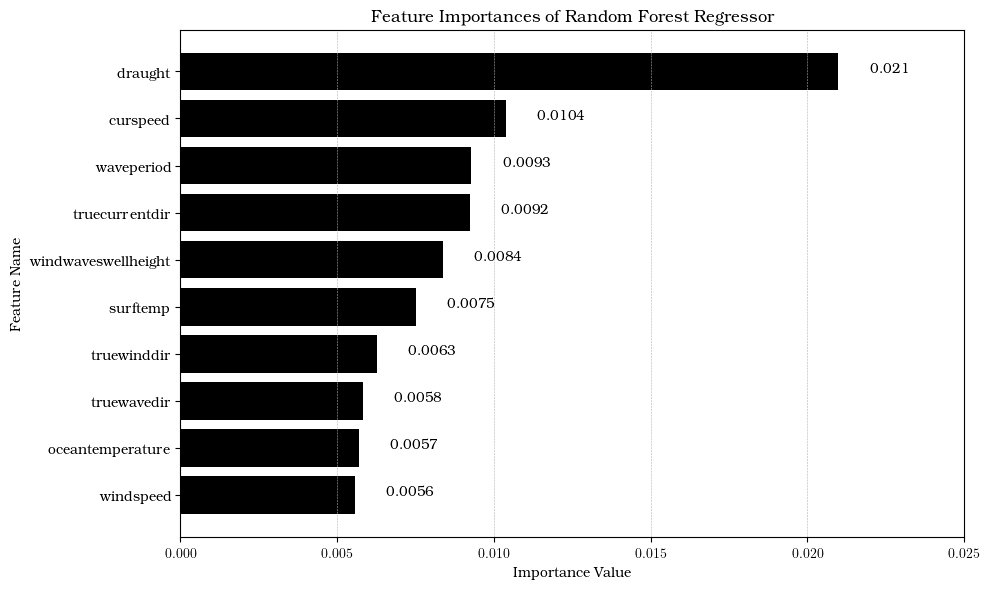
\includegraphics[width=.9\textwidth]{02_figures/rfr_ftr_importance_nodir.png}
%         \caption{Feature importance of RFR}
%         \label{fig:ftr_impo_rfr}
% \end{figure}

% \begin{figure}[h]
%     \centering
%         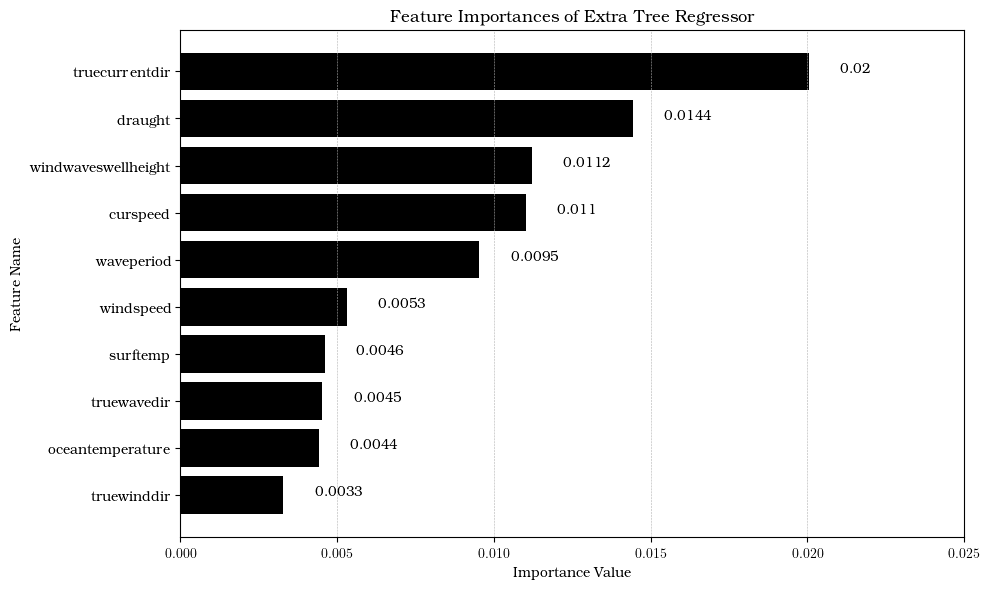
\includegraphics[width=.9\textwidth]{02_figures/etr_ftr_importance_nodir.png}
%         \caption{Feature importance of ETR}
%         \label{fig:ftr_impo_etr}
% \end{figure}

Excluding ship heading and COG. The ship draught $T$ emerges as a significant factor influencing the prediction of SOG. This aligns with the theory of frictional resistance $R_F$ encountered by the ship, which is discussed in \Cref{sec:Calm_Resistance}. \Cref{eqn:R_f} is a function of wetted surface area of bare hull $S$. Deeper draught $T$ will result in more submerged area of the hull and this will consequently increase the frictional force $R_F$ of the ship. Given a constant supply of power to the ship propulsion system, the speed of the ship will decrease which is shown in \Cref{eqn:P_e}.\\

\pagebreak

Concerning weather states, both the RFR and ETR models identify current-based information, such as current speed and true current direction, as the most influential factors affecting SOG prediction. This observation concurs with the suggested methodology for current correction presented in Section \Cref{sec:SOG_corr}, which outlines that the process of converting SOG to STW necessitates both the magnitude and direction of the current. The subsequent influential features, according to the rankings of the RFR and ETR models, are wave-related attributes: significant wave height ($H_{1/3}$), true wave direction, and wave period ({\tt waveperiod}). This alignment reflects the added resistance caused by waves ($R_{AW}$) in the computation of the total resistance ($R_{TOTAL}$) experienced by the ship. On the other hand, wind-related features, encompassing wind speed and its true direction, are associated with the added resistance due to wind force ($R_{AA}$). However, these factors are found to be the least impactful in the prediction of SOG according to the RFR and ETR models.\\

Based on the behaviour of the Random Forest Regressor (RFR) and Extra Trees Regressor (ETR) models, it can be inferred that waves have a more significant impact on the Speed Over Ground (SOG) compared to the influence of wind during the ship's journey. However, the Decision Tree Regressor (DTR) model demonstrates that temperature-related features, such as Sea Surface Temperature (SST) and air temperature above the ocean, have a more significant effect on SOG predictions than most other features. While the importance of temperature is not as pronounced as in RFR or ETR models, this finding suggests that the ship's SOG is implicitly influenced by the time of the travel or the season in which the journey takes place.\\

\subsubsection*{Structure of generated tree-based model}

% \begin{figure}[h]
%     \centering
%         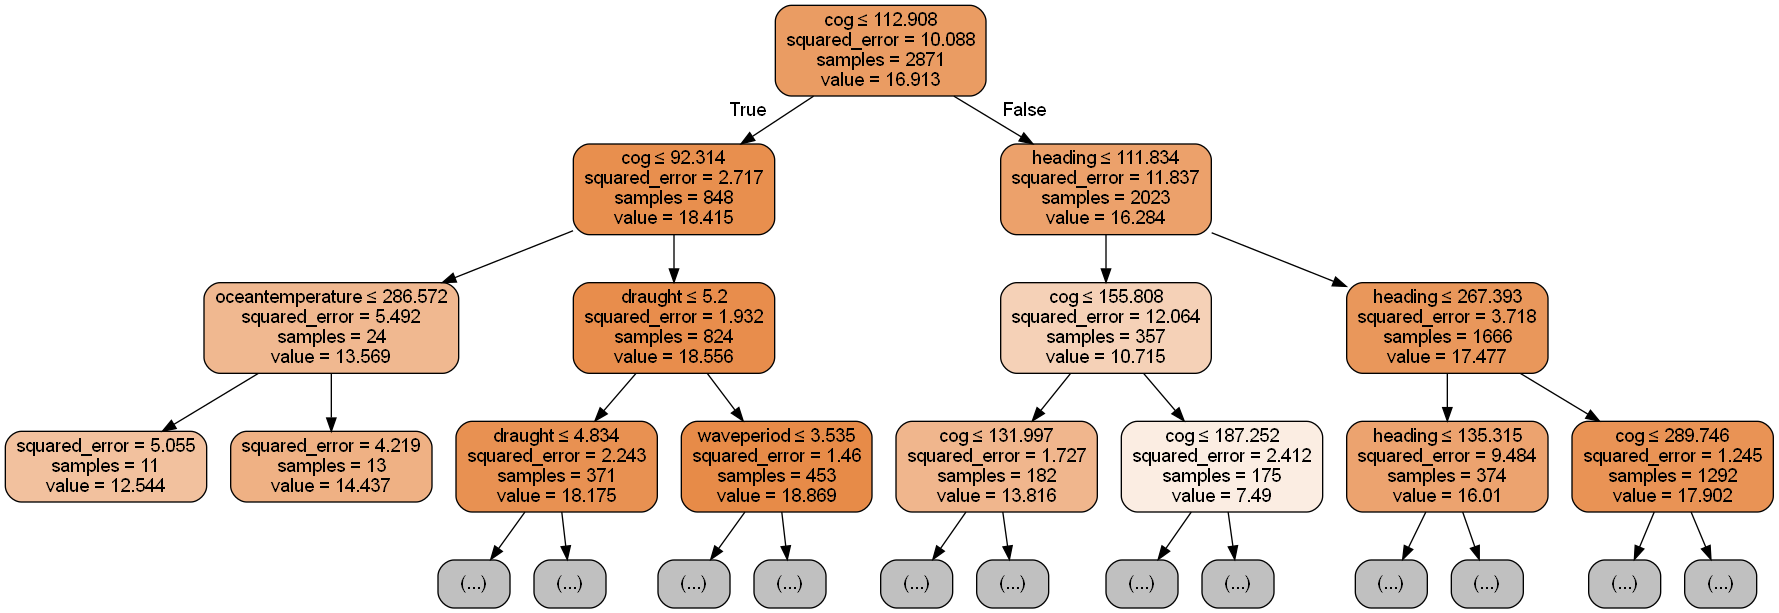
\includegraphics[width=.9\textwidth]{02_figures/dtr_mod_1tree.png}
%         \caption{Partial structure of DTR}
%         \label{fig:dtr_tree_hpov}
% \end{figure}

To comprehend the impact of hyperparameter optimisation and feature importance, an analysis of the structure of the generated tree-based models will be conducted. The shading within the nodes conveys the probability of the decision, with darker shading indicating a higher likelihood. Each node provides information about the splitting feature, along with its threshold, SSR (Sum of Squared Residuals) value, sample count, and the predicted SOG value. Despite pruning efforts, the tree structure can potentially become quite large. To enhance clarity, the visualization of the trees will be restricted to a maximum depth of {\tt max\_depth = 3}. Additionally, for the RFR and ETR models, only the illustration of a specific tree within the forest will be presented.\\

The structure of the optimized decision tree, as depicted in \Cref{fig:overall_tree_partial_structure}, illustrates the impact of regularisation at the leaf nodes. Notably, the leaf nodes that partition the feature ocean temperature do not achieve a complete minimization of the SSR. This outcome arises from the hyperparameter tuning of the minimum samples at the leaf nodes, set at {\tt min\_samples\_leaf = 10}. Further division of these nodes would result in subsequent leaf nodes with fewer than 10 samples. Within this visualisation, the significance of features such as COG and ship heading becomes evident, as they are employed to partition numerous internal nodes in the tree.\\

% \begin{figure}[h]
%     \centering
%         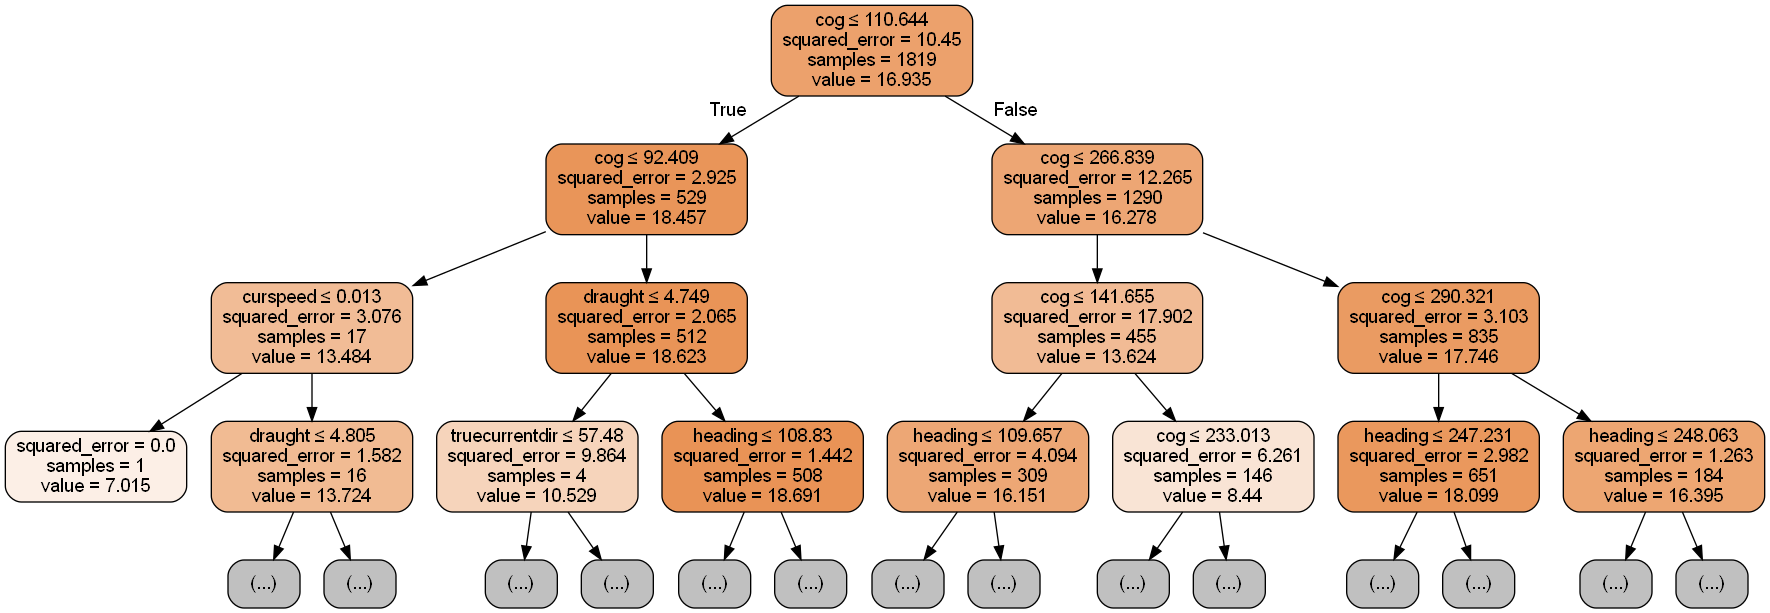
\includegraphics[width=.9\textwidth]{02_figures/rfr_mod_it1.png}
%         \caption{Partial structure of {\tt n\_estimators = 1} for RFR}
%         \label{fig:rfr_tree1_hpov}
% \end{figure}

The illustration of the first RFR tree is shown in \Cref{fig:overall_tree_partial_structure}. Similar to DTR, both COG and ship heading are regarded as the best features to split the internal node. In this tree of the forest, the effect of allowing full tree growth can be observed in the leaf node when splitting the feature current speed. This tree is able to minimise the SSR to its possible minimum value, and the leaf node cannot be further split as there are no more available samples. The effect of bagging for the dataset and feature selection in RFR can also be observed in this tree as the structure of this tree is completely different to DTR tree shown in \Cref{fig:overall_tree_partial_structure}.\\

% \begin{figure}[h]
%     \centering
%         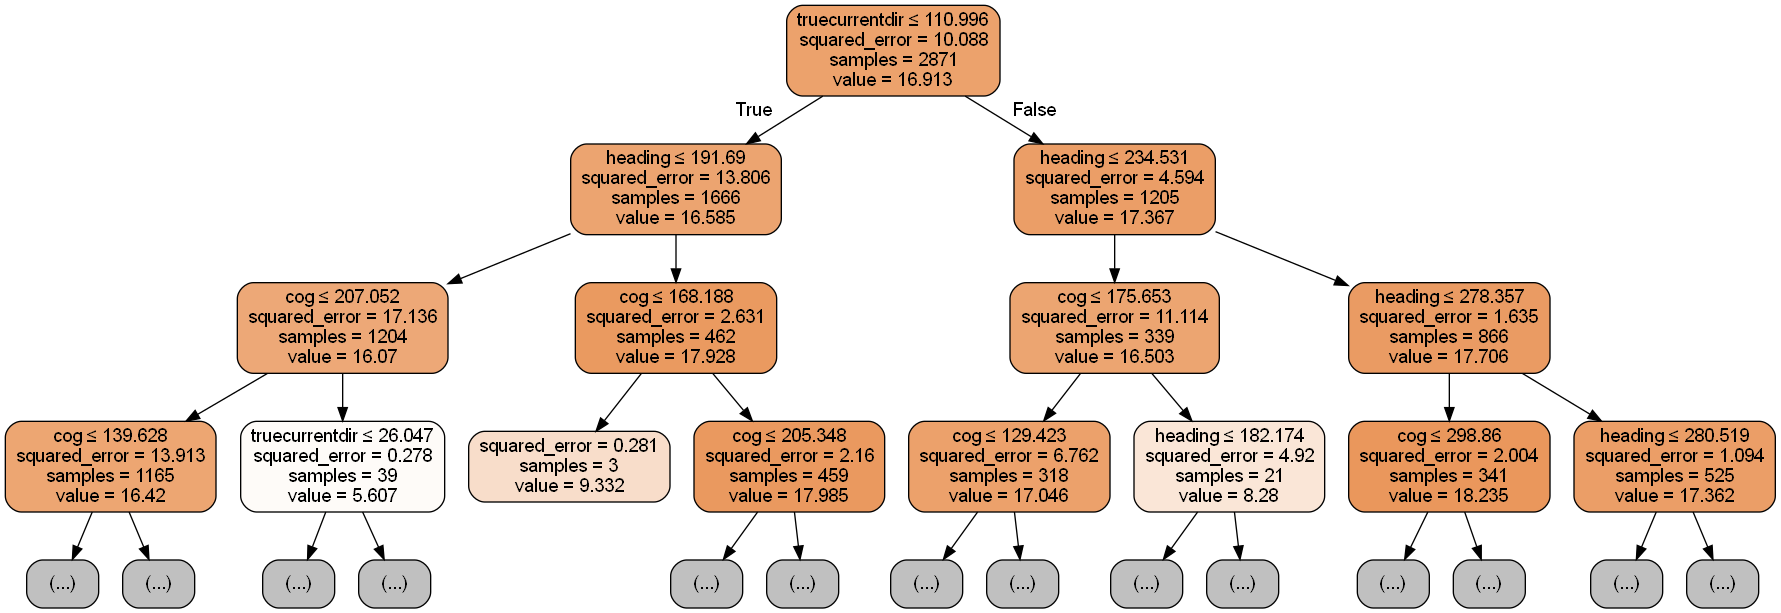
\includegraphics[width=.9\textwidth]{02_figures/etr_mod_it1.png}
%         \caption{Partial structure of {\tt n\_estimators = 1} for ETR}
%         \label{fig:etr_tree1_etr}
% \end{figure}

\begin{figure}
    \centering
    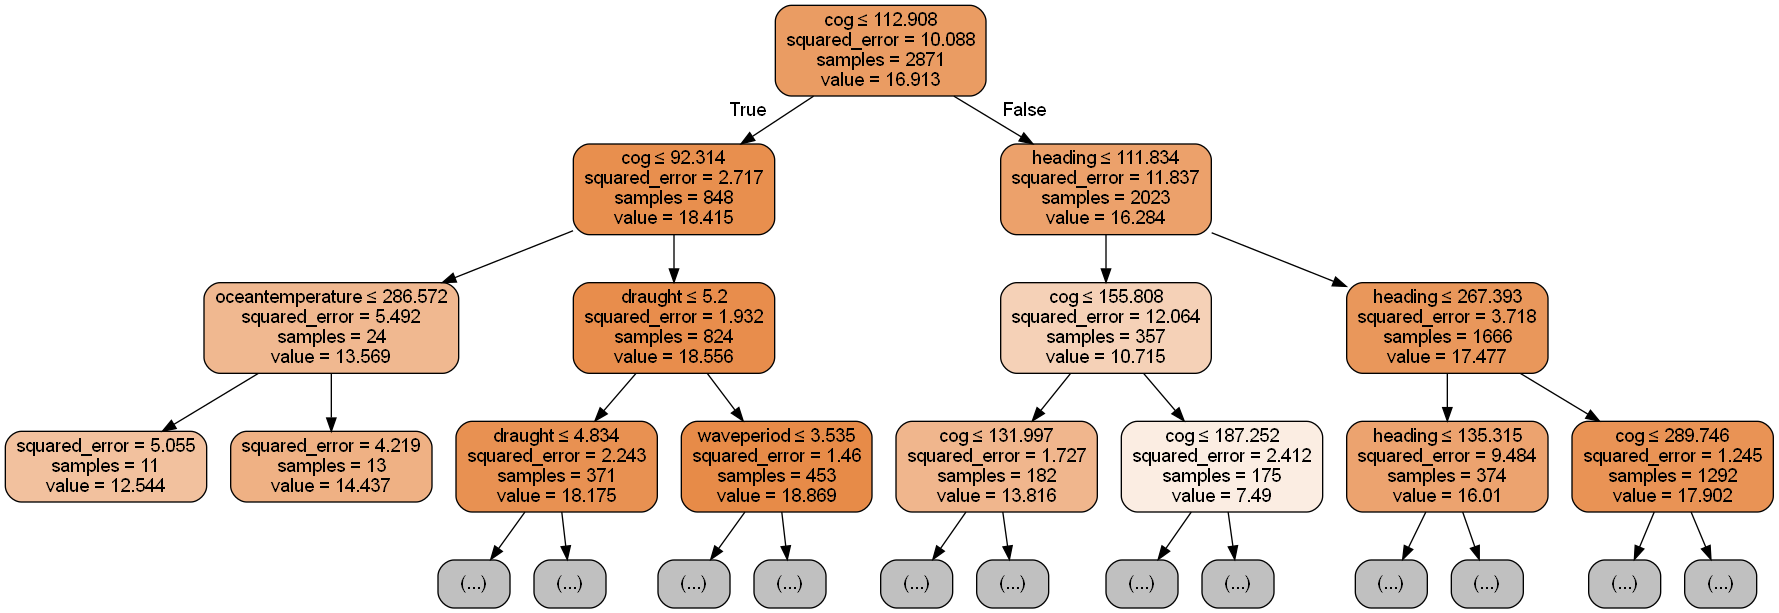
\includegraphics[width=.9\textwidth]{02_figures/dtr_mod_1tree.png}\\
    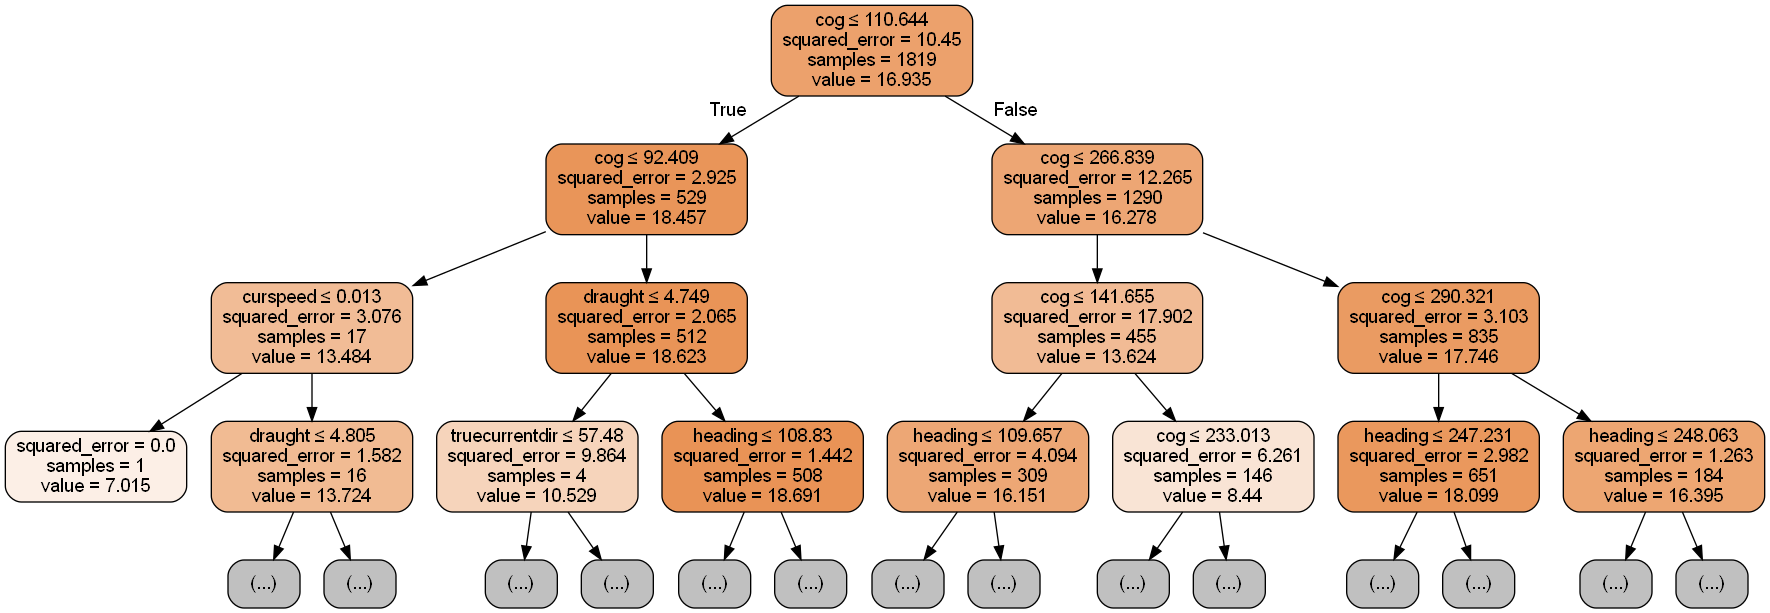
\includegraphics[width=.9\textwidth]{02_figures/rfr_mod_it1.png}\\
    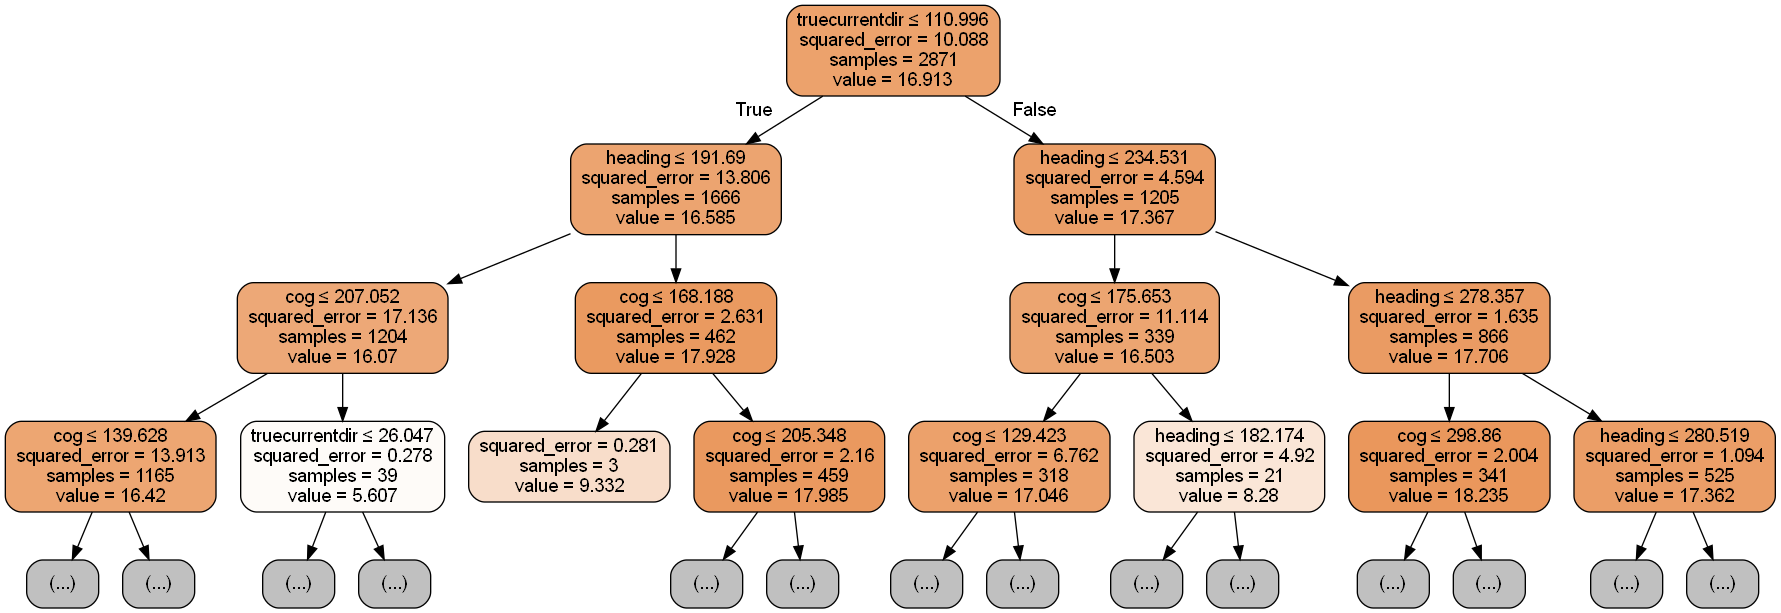
\includegraphics[width=.9\textwidth]{02_figures/etr_mod_it1.png}
    \caption{Partial structure of DTR, RFR, and ETR}
    \label{fig:overall_tree_partial_structure}
\end{figure}

The influence of random feature selection in ETR is demonstrated by the structure of its first tree, as presented in \Cref{fig:overall_tree_partial_structure}. Unlike the DTR and RFR, which employ a greedy algorithm to identify splits minimizing the cost function, the ETR exhibits a noticeable randomness in feature selection. In this specific illustration, the ETR model designates the true current direction as the parent node. Furthermore, due to the regularisation applied to the ETR, the leaf node formed during the COG split does not entirely minimize the SSR. It is worth noting that this particular split does not occur due to the constraint imposed by the tuning parameter {\tt min\_samples\_split = 9}.\\

\subsubsection{Evaluation of k-fold cross-validation}\label{sec:bbm_kfold_perf_eval}

The results of the 10-fold validation process are shown in \Cref{fig:k_fold_validation_result}. The inner (orange) line corresponds to the median, representing the central $50\%$ of scores in the k-folding procedure. The upper and lower boundaries of the box signify the first ($25\%$) and third ($75\%$) quartiles, respectively. The whiskers denote the lowest data point within a 1.5 Interquartile Range (IQR) of the lower quartile and the highest data point within a 1.5 IQR of the upper quartile. The mean value is indicated by the (green) triangle, while data points beyond the whisker range are depicted as hollow circles.\\

\begin{figure}[ht]
    \centering
  
    \begin{minipage}{0.45\textwidth}
      \centering
      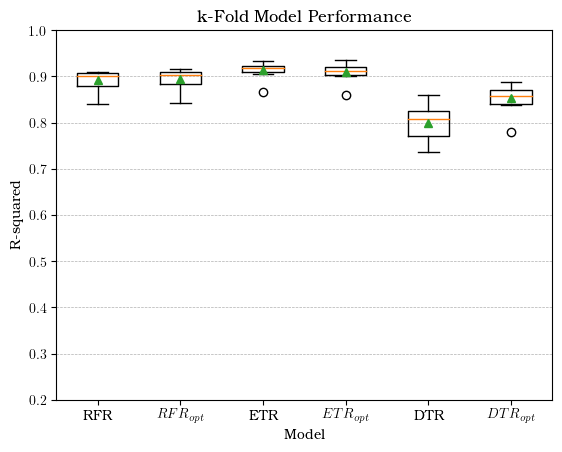
\includegraphics[width=\textwidth]{02_figures/kfold_r2_opt.png}
    \end{minipage}
    \hfill
    \begin{minipage}{0.45\textwidth}
      \centering
      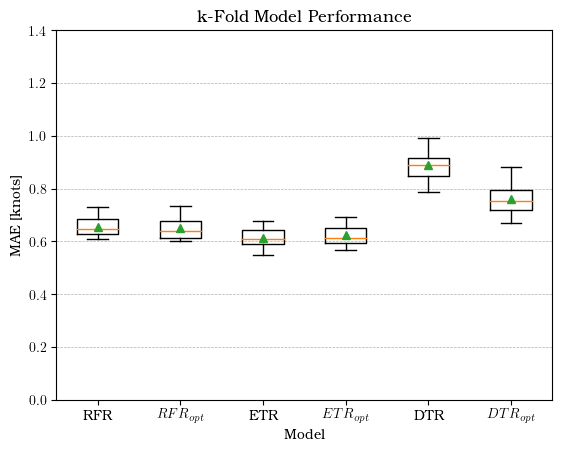
\includegraphics[width=\textwidth]{02_figures/kfold_mae_opt.png}
    \end{minipage}
  
    \vspace{0.1cm} % Adjust the vertical space between rows
  
    \begin{minipage}{0.45\textwidth}
      \centering
      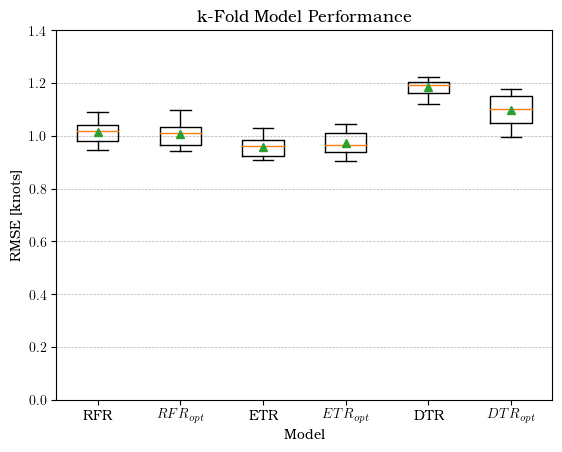
\includegraphics[width=\textwidth]{02_figures/kfold_rmse_opt.png}
    \end{minipage}
    \hfill
    \begin{minipage}{0.45\textwidth}
      \centering
      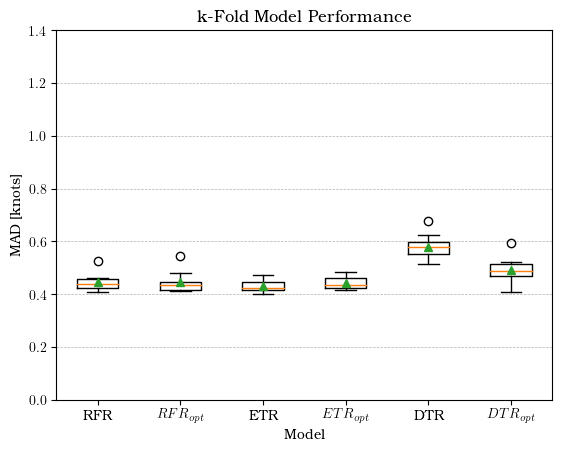
\includegraphics[width=\textwidth]{02_figures/kfold_mad_opt.png}
    \end{minipage}
  
    \caption{Evaluation of k-fold cross-validation for different performance indices}
    \label{fig:k_fold_validation_result}
  \end{figure}

The box plots reveal that ETR outperformed other tree-based models, achieving a $R^2$ score of approximately $91\%$ and an MAE of around 0.6 knots. This model also demonstrated notable stability, evident from the narrow length between the first and third quartile. RFR showcased a similar level of performance, attaining an $R^2$ score of roughly $89\%$ and an MAE of about 0.65 knots. As demonstrated previously in \Cref{fig:learn_curve_TREE_MAE}, hyperparameter optimization did not lead to any substantial enhancement in model performance. DTR significantly benefited from the process of regularisation, resulting in an increase of around $5\%$ in the $R^2$ score and a reduction in MAE from about 0.89 knots to 0.76 knots. Similar improvements can be observed in both RMSE and MAD. In summary, all tree-based models demonstrated a satisfactory fit, with mean/median $R^2$ scores exceeding $80\%$. However, the RMSE values are relatively significant, ranging from 1.00 to 1.20 knots across the models. To provide context, the mean SOG of the training data is 16.91 knots, as indicated in \Cref{tbl:dataset_descriptive_pretraining}.\\

\subsection{Performance evaluation of BBM}\label{sec:Perf_eval_BBM}

\subsubsection{Analysing the testing dataset}\label{sec:testing_data_analysis}

Once the best-optimised model is identified, the performance of the model will be further evaluated using the testing dataset. This testing dataset comprises 957 data points from the year 2021, encompassing the entirety of the year. The dataset for the full year is denoted as $DS_{year}$. In order to explore the influence of data points on model performance, the dataset is divided into two distinct seasons: $DS_{summer}$, covering the period from May 2021 to October 2021, consisting of 454 data points; and $DS_{winter}$, encompassing data from January 2021 to April 2021, as well as November 2021 to December 2021, with a total of 503 data points. Any missing values present within the testing dataset will be addressed using the {\tt KNNImputer} method.\\

\begin{table}[h!]
    \footnotesize
    \centering
    % \resizebox {\textwidth}{!}
    {\begin{tabular}{ p{0.21\linewidth} c c c c c c c c }
    \hline
    Features & Count & Mean & Std. & Min & 25\% & 50\% & 75\% & Max \\
    \hline
    \textbf{{\tt sog}} & 957.00 & 16.99 & 3.10 & 5.10 & 16.68 & 18.05 & 18.72 & 21.00\\
    \hline
    {\tt cog} & 957.00 & 196.73 & 86.72&	56.02 & 102.32& 185.22& 282.18& 319.85\\ 
    {\tt heading} & 957.00 & 188.30&	89.17&	63.49&	100.86&	124.24&	279.38&	308.04\\
    {\tt draught} & 957.00 & 5.23 & 0.19& 4.74& 5.11& 5.29& 5.38&5.66\\
    {\tt windspeed} & 957.00 & 6.45 & 3.04 & 0.40 & 4.11 & 6.13 &	8.21 & 15.85\\
    {\tt oceantemperature} & 957.00 & 282.28 & 6.48 & 267.25& 276.80& 281.91& 288.42& 295.70 \\
    {\tt waveperiod} & 957.00 & 3.70 & 0.88 & 1.67 & 3.06& 3.62& 4.22& 7.01\\
    {\tt surftemp} & 957.00 &283.22& 5.72& 273.15& 277.98& 282.73& 288.82 &294.93\\
    {\tt windwaveswellheight} &  957.00 & 0.77 & 0.54 & 0.08 &0.37 &	0.66 &	0.94 &  3.24  \\
    {\tt curspeed} & 957.00 &0.09 & 0.07& 0.00 & 0.05& 0.07 & 0.13 & 0.50\\
    {\tt truewinddir} & 957.00 & 91.39 & 56.23 &	0.03 & 38.80 &	95.25 & 142.83 & 179.86\\
    {\tt truecurrentdir} & 957.00 & 90.75 & 57.76 & 0.26 & 31.52 & 90.44 & 144.65 & 179.95 \\
    {\tt truewavedir} & 957.00 & 86.90 & 55.74& 0.06& 36.24 & 81.54 & 138.04 & 179.81 \\
    \hline
    \end{tabular}}
\caption{Descriptive statistics of $DS_{year}$}\label{tbl:testyear_dataset_descriptive}
\end{table}

\begin{table}[h!]
    \footnotesize
    \centering
    % \resizebox {\textwidth}{!}
    {\begin{tabular}{ p{0.21\linewidth} c c c c c c c c }
    \hline
    Features & Count & Mean & std & Min & 25\% & 50\% & 75\% & Max \\
    \hline 
    \textbf{{\tt sog}} & 454.00 & 17.26 & 2.91 & 5.22 & 16.74 & 18.17 & 18.95 & 21.01\\
    \hline
    {\tt cog} & 454.00 & 196.06 & 87.55 &  56.02 & 102.80 & 182.79 & 282.03 & 319.85 \\ 
    {\tt heading} & 454.00 & 188.08 & 89.02 &  63.49 & 100.75 & 124.68 & 278.07 & 303.30 \\
    {\tt draught} & 454.00 &   5.30 &  0.17 &   4.74 &   5.20 &   5.29 &   5.38 &   5.66 \\
    {\tt windspeed} & 454.00 &   6.64 &  3.33 &   0.40 &   4.08 &   6.30 &   8.71 &  15.85 \\
    {\tt oceantemperature} & 454.00 & 285.59 &  5.90 & 269.27 & 282.90 & 286.70 & 290.04 & 295.70 \\
    {\tt waveperiod} & 454.00 & 3.73 &  0.99 &   2.02 &   2.95 &   3.60 &   4.36 &   7.01 \\
    {\tt surftemp} & 454.00 & 286.33 &  5.10 & 274.75 & 283.05 & 287.58 & 290.18 & 294.93 \\
    {\tt windwaveswellheight} & 454.00 &   0.82 &  0.63 &   0.08 &   0.36 &   0.67 &   1.02 &   3.24 \\
    {\tt curspeed} & 454.00 &   0.10 &  0.07 &   0.00 &   0.04 &   0.07 &   0.13 &   0.50 \\
    {\tt truewinddir} & 454.00 &  90.94 & 58.05 &   0.60 &  38.40 &  89.86 & 145.86 & 179.58 \\
    {\tt truecurrentdir} & 454.00 &  83.65 & 59.53 &   0.26 &  26.68 &  70.51 & 143.73 & 179.33 \\
    {\tt truewavedir} & 454.00 &  88.06 & 59.52 &   0.09 &  33.00 &  82.18 & 145.69 & 179.81 \\
    \hline
    \end{tabular}}
\caption{Descriptive statistics of $DS_{summer}$}\label{tbl:testsummer_dataset_descriptive}
\end{table}

\begin{table}[h!]
    \footnotesize
    \centering
    % \resizebox {\textwidth}{!}
    {\begin{tabular}{ p{0.21\linewidth} c c c c c c c c }
    \hline
    Features & Count & Mean & std & Min & 25\% & 50\% & 75\% & Max \\
    \hline
    \textbf{{\tt sog}} & 503.00 & 16.75 & 3.24 & 5.10 & 16.59 & 17.98 & 18.61 & 20.70\\
    \hline
    {\tt cog} & 503.00 & 197.33 & 86.06 &  80.81 & 102.25 & 187.56 & 282.63 & 307.92 \\
    {\tt heading} & 503.00 & 188.50 & 89.39 &  89.22 & 100.87 & 123.92 & 280.05 & 308.04 \\
    {\tt draught} & 503.00 &   5.16 &  0.18 &   4.76 &   5.02 &   5.20 &   5.29 &   5.65 \\
    {\tt windspeed}& 503.00 &   6.28 &  2.76 &   0.43 &   4.12 &   6.05 &   8.01 &  14.35 \\
    {\tt oceantemperature} & 503.00 & 279.29 &  5.44 & 267.25 & 275.74 & 278.22 & 281.25 & 292.72 \\
    {\tt waveperiod} & 503.00 & 3.67 &  0.76 &   1.67 &   3.16 &   3.62 &   4.14 &   5.98 \\
    {\tt surftemp} & 503.00 & 280.41 &  4.71 & 273.15 & 277.23 & 278.68 & 282.68 & 292.85 \\
    {\tt windwaveswellheight} & 503.00 &   0.73 &  0.45 &   0.08 &   0.40 &   0.66 &   0.90 &   2.43 \\
    {\tt curspeed} & 503.00 &   0.09 &  0.07 &   0.00 &   0.05 &   0.08 &   0.12 &   0.42 \\
    {\tt truewinddir} & 503.00 &  91.81 & 54.61 &   0.03 &  39.66 &  97.92 & 140.20 & 179.86 \\
    {\tt truecurrentdir} & 503.00 &  97.16 & 55.40 &   1.44 &  41.92 & 102.12 & 145.34 & 179.95 \\
    {\tt truewavedir} & 503.00 &  85.86 & 52.13 &   0.06 &  39.44 &  81.22 & 132.49 & 178.30 \\
    \hline
    \end{tabular}}
\caption{Descriptive statistics of $DS_{winter}$}\label{tbl:testwinter_dataset_descriptive}
\end{table}

\clearpage

\subsubsection{Result and Discussion of BBM}\label{sec:result_discussion_BBM}

The results of SOG prediction of optimised tree-based models are summarised in \Cref{tbl:testing_dataset_sog_result}. Each model is tested against 3 different testing datasets, the yearly dataset $DS_{year}$, summer dataset, $DS_{summer}$ and winter dataset $DS_{winter}$. The performance of the tree models is compared against Multiple Linear Regressor (MLR) model.

\begin{table}[ht]
    \footnotesize
    % \small
    \centering
    % \resizebox {\textwidth}{!}
    {\begin{tabular}{ l l c c c c c c }
    \hline
    Model & Dataset & $R^2$ & expVar & MAE & RMSE & MAD & MAPE \\
    & & [$\%$] & [$\%$] & [$kn$] & [$kn$] & [$kn$] & [$\%$]  \\ 
    \hline
    $\text{DTR}_{OPT}$ & $DS_{year}$ & 86.72 & 86.75 & 0.714 & 1.129  & 0.479 & 4.96  \\
    & $DS_{winter}$ & 88.51 & 88.61 & 0.690 & 1.100 & 0.441 & 4.95 \\
    & $DS_{summer}$ & 84.04 & 84.05 & 0.741 & 1.161 & 0.520 & 4.97 \\
    $\text{RFR}_{OPT}$ & $DS_{year}$  & 90.13 & 96.16 & 0.629 & 0.973 & 0.419 & 4.29 \\
    & $DS_{winter}$ & 93.40 & 93.52 & 0.549 & 0.833 & 0.374 & 3.96 \\
    & $DS_{summer}$ & 85.48 & 85.48 & 0.696 & 1.108 & 0.455 & 4.66 \\
    $\text{ETR}_{OPT}$ & $DS_{year}$ & 91.09 & 91.91 & 0.582 & 0.882 & 0.398 & 3.96 \\
    & $DS_{winter}$ & \textbf{94.55} & \textbf{94.63} & \textbf{0.532} & \textbf{0.756} & \textbf{0.394} & \textbf{3.72} \\
    & $DS_{summer}$ & 88.11 & 88.13 & 0.637 & 1.002 & 0.409 & 4.23 \\
    MLR & $DS_{year}$ & 69.61 & 69.67 & 1.147 & 1.707 & 0.924 & 7.73 \\
    & $DS_{winter}$ & 68.08 & 68.08 & 1.135 & 1.831 & 0.880 & 8.04 \\
    & $DS_{summer}$ & 71.21 & 71.56 & 1.160 & 1.560 & 0.949 & 7.39 \\
    \hline
    \end{tabular}}
\caption{Performance indices for SOG predictions}\label{tbl:testing_dataset_sog_result}
\end{table}

The results presented in \Cref{tbl:testing_dataset_sog_result} shows that all tree-based models demonstrated good predictive capabilities across various testing datasets. Generally, all tree-based models obtained $R^2$ score above $80\%$ and perform better when using the $DS_{winter}$ datasets. All tree-based models offer a substantial improvement from MLR. Among the tree-based model, ETR presented the best SOG prediction across different datasets, closely followed by RFR and followed by  DTR.\\ 

\begin{table}[h]
    \footnotesize
    \centering
    % \resizebox {\textwidth}{!}
    {\begin{tabular}{ l l c c c c c c c c }
    \hline
    Model & Dataset & Count & Mean & std & Min & 25\% & 50\% & 75\% & Max \\
    \hline
    \textbf{{Actual}} & $DS_{year}$ & 957.00 &  16.99 &   3.10 & 5.10 &  16.68 &  18.05 &  18.72 &  21.01 \\
    & $DS_{winter}$ & 503.00 &  16.75 &   3.24 & 5.10 &  16.59 &  17.98 &  18.61 &  20.70 \\
    & $DS_{summer}$ & 454.00 &  17.26 &   2.91 & 5.22 &  16.74 &  18.17 &  18.95 &  21.01 \\
    $\text{DTR}_{OPT}$ & $DS_{year}$ & 957.00 &  17.04 &   2.91 & 5.36 &  16.58 &  18.11 &  18.66 &  20.00 \\
    & $DS_{winter}$ & 503.00 &  16.85 &   3.06 & 5.36 &  16.58 &  17.86 &  18.58 &  19.98 \\
    & $DS_{summer}$ & 454.00 &  17.25 &   2.73 & 5.64 &  16.58 &  18.15 &  18.91 &  20.00 \\
    $\text{RFR}_{OPT}$ & $DS_{year}$ & 957.00 &  17.04 &   2.89 & 5.37 &  16.71 &  18.11 &  18.70 &  20.22 \\
    & $DS_{winter}$ & 503.00 &  16.86 &   3.04 & 5.37 &  16.70 &  18.02 &  18.60 &  19.74 \\
    & $DS_{summer}$ & 454.00 &  17.25 &   2.72 & 5.81 &  16.74 &  18.20 &  18.77 &  20.22 \\
    $\text{ETR}_{OPT}$ & $DS_{year}$ & 957.00 &  17.03 &   2.87 & 5.39 &  16.67 &  18.05 &  18.65 &  19.96 \\
    & $DS_{winter}$ & 503.00 &  16.84 &   3.04 & 5.39 &  16.65 &  17.96 &  18.56 &  19.87 \\
    & $DS_{summer}$ & 454.00 &  17.23 &   2.66 & 5.96 &  16.71 &  18.18 &  18.75 &  19.96 \\
    \hline
    \end{tabular}}
\caption{Descriptive statistics of SOG Prediction}\label{tbl:SOG_pred_descriptive}
\end{table}

% \begin{figure}[ht]
% \centering

% \begin{minipage}[b]{0.32\textwidth}
%     \centering
%     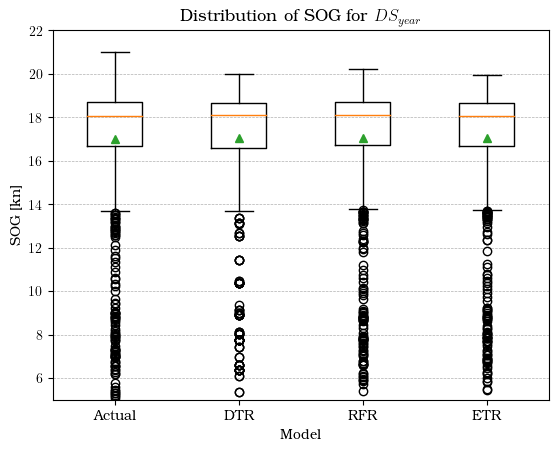
\includegraphics[width=\textwidth]{02_figures/sog_pred_year.png}
%     % \caption{Caption for Picture 1.}
%     \label{fig:boxplot_dsyear}
% \end{minipage}%
% \hfill
% \begin{minipage}[b]{0.32\textwidth}
%     \centering
%     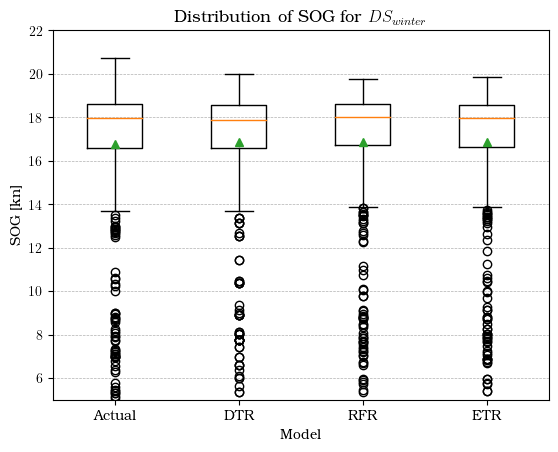
\includegraphics[width=\textwidth]{02_figures/sog_pred_winter.png}
%     % \caption{Caption for Picture 2.}
%     \label{fig:boxplot_dswinter}
% \end{minipage}%
% \hfill
% \begin{minipage}[b]{0.32\textwidth}
%     \centering
%     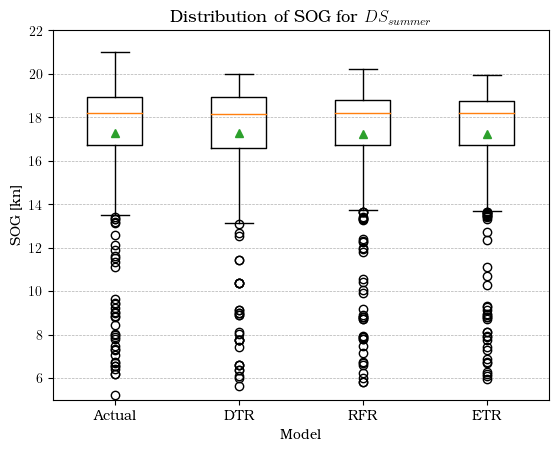
\includegraphics[width=\textwidth]{02_figures/sog_pred_summer.png}
%     % \caption{Caption for Picture 3.}
%     \label{fig:boxplot_dssummer}
% \end{minipage}

% \caption{SOG distribution for $DS_{year}$, $DS_{winter}$ and $DS_{summer}$}
% \label{fig:boxplot_sogPred_overall}
% \end{figure}  

\begin{figure}[h!]
    \centering
        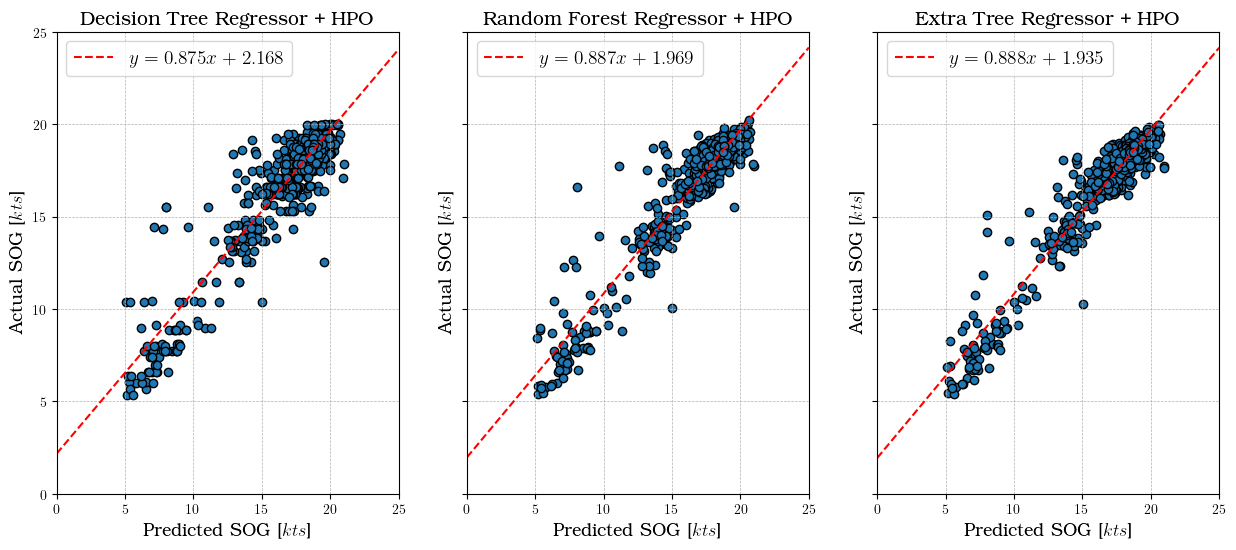
\includegraphics[width=.9\textwidth]{02_figures/pred_vs_act_all_tree.png}
        \caption{Actual vs Predicted SOG for DTR, RFR and ETR}
        \label{fig:pred_vs_act_SOG}
\end{figure}

\begin{figure}
    \centering
        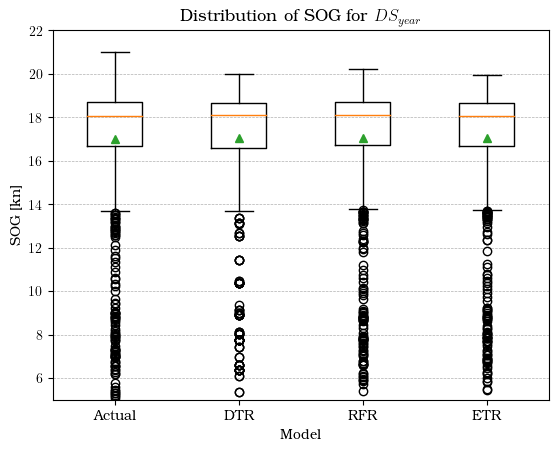
\includegraphics[width=.75\textwidth]{02_figures/sog_pred_year.png}
        \caption{SOG distribution for $DS_{year}$}
        \label{fig:boxplot_sogPred_yr}
\end{figure}

For a deeper understanding of predictive performance, descriptive statistics of the SOG prediction are presented in \Cref{tbl:SOG_pred_descriptive}. The results suggest that the model struggles to capture information at lower ship speeds across the various datasets. This limitation could potentially be caused by the scarcity of data points representing the lower end of SOG. Such sparsity is evident from the boxplots of diverse datasets depicted in \Cref{fig:boxplot_sogPred_yr}, as well as the actual versus predicted SOG plot illustrated in \Cref{fig:pred_vs_act_SOG}, where the scarcity of information in lower SOG range data points becomes notably evident.\\

% \begin{figure}
%     \centering
%         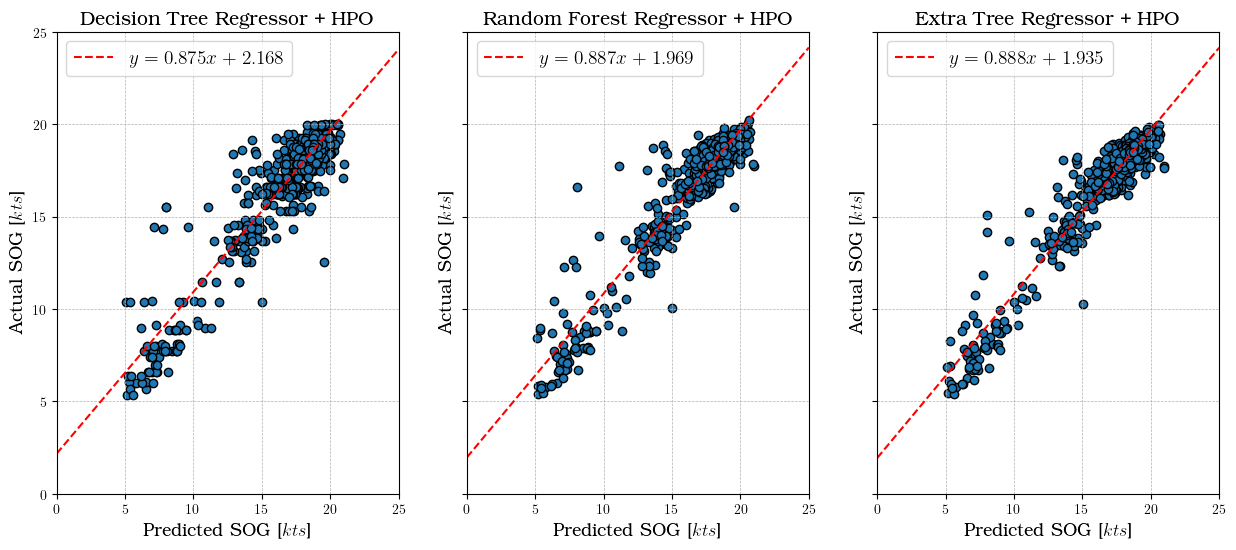
\includegraphics[width=.9\textwidth]{02_figures/pred_vs_act_all_tree.png}
%         \caption{Actual vs Predicted SOG for DTR, RFR and ETR}
%         \label{fig:pred_vs_act_SOG}
% \end{figure}

Both the descriptive statistics and boxplots indicate that the distribution of data points is skewed towards higher SOG values. The majority of data points cluster around approximately 16.5 knots for the first quartile and 19 knots for the third quartile, which is consistently observed across all datasets. The lowest data point within the $1.5 \cdot \text{IQR}_{LOW}$ range is situated around 13.6 knots, as evident from the lower whisker in the boxplot. Despite the appearance of potential outliers beyond the whisker in the boxplot, these points do not signify actual outliers; instead, they represent ship journeys at low speeds. The limited representation of low-speed data points contributes to the model's challenge in accurately predicting SOG values within the lower SOG range.\\

This observation could potentially explain the relatively high values of RMSE for all the models. As discussed earlier in \Cref{sec:perf_metrics}, RMSE is more sensitive to outliers compared to both MAE and MAD, which makes it less suitable for this case study. In contrast, MAE and MAD provide more robust error evaluation metrics in situations like this. Additionally, the elevated $R^2$ scores and explained variance could be attributed to the models' effectiveness in predicting SOG values that fall within the interquartile ranges indicated by the boxplot whiskers. This suggests strong prediction performance within those specific ranges.\\

\pagebreak

There are two possible solutions to address this problem:\\ 

\textbf{Increasing the number of data points in the lower SOG Range}: This is the most apparent solution to address this issue. By doing so, the interquartile range (IQR) of the boxplot can be expanded, potentially preventing the misclassification of lower SOG data points as outliers. Furthermore, this could lead to improvements in performance metrics such as $R^2$ and RMSE. However, it is important to note that in the context of this specific case study, this approach may not be feasible due to the limitations of T-AIS coverage, as illustrated in \Cref{fig:aiscoverage}. The ship's speed decrease as it approaches a port and it gradually increases as it departs from one. Unfortunately, T-AIS coverage around the ports of K{\o}ge and R{\o}nne is either problematic, with a transmission and reception rate of approximately 50\% to 80\%, or poor, with a transmission rate of less than 50\%. This presents a significant challenge, as increasing the number of data points around these port regions may not be achievable given the limitations of T-AIS transmission rates.\\

\textbf{Reducing data Skewness}: A strategy to address data skewness could involve applying outlier rejection techniques, as demonstrated by \citet{Gkerekos.2019}. The outlier rejection formula $\mu \pm 3\sigma$, where $\mu$ is the mean and $\sigma$ is the standard deviation, could be employed. Assuming a normal distribution, this range should encompass approximately $99.7\%$ of the normal data. Another approach to mitigate skewness is to set a higher threshold for the minimum SOG value. While this might lead to an overall reduction in errors and an improvement in model fit, it's important to note that such an approach could limit the model's ability to make accurate predictions when the ship is operating at lower speeds. Careful consideration of the trade-offs between model performance and predictive capability is essential when determining the most suitable approach. The effect of reducing skewness on the testing datasets will be demonstrated in subsequent sections.\\

\section{Evaluation of WBM}\label{sec:WBM_perf_eval}

\subsection{Analysis of WBM}\label{sec:Power_estimation_actual}

The findings of power estimation using the Holtrop-Mennen method are presented in \Cref{tbl:PB_act_descriptive_yr} and \Cref{fig:hist_resistance_power_yr}. To gain insights into the overall model behaviour, the analysis is conducted using the actual data from the $DS_{year}$ datasets. To facilitate a better interpretation of the scale of magnitude, the histograms for the resistance components utilise identical scaling.\\

\begin{figure}[h!]
    \centering
    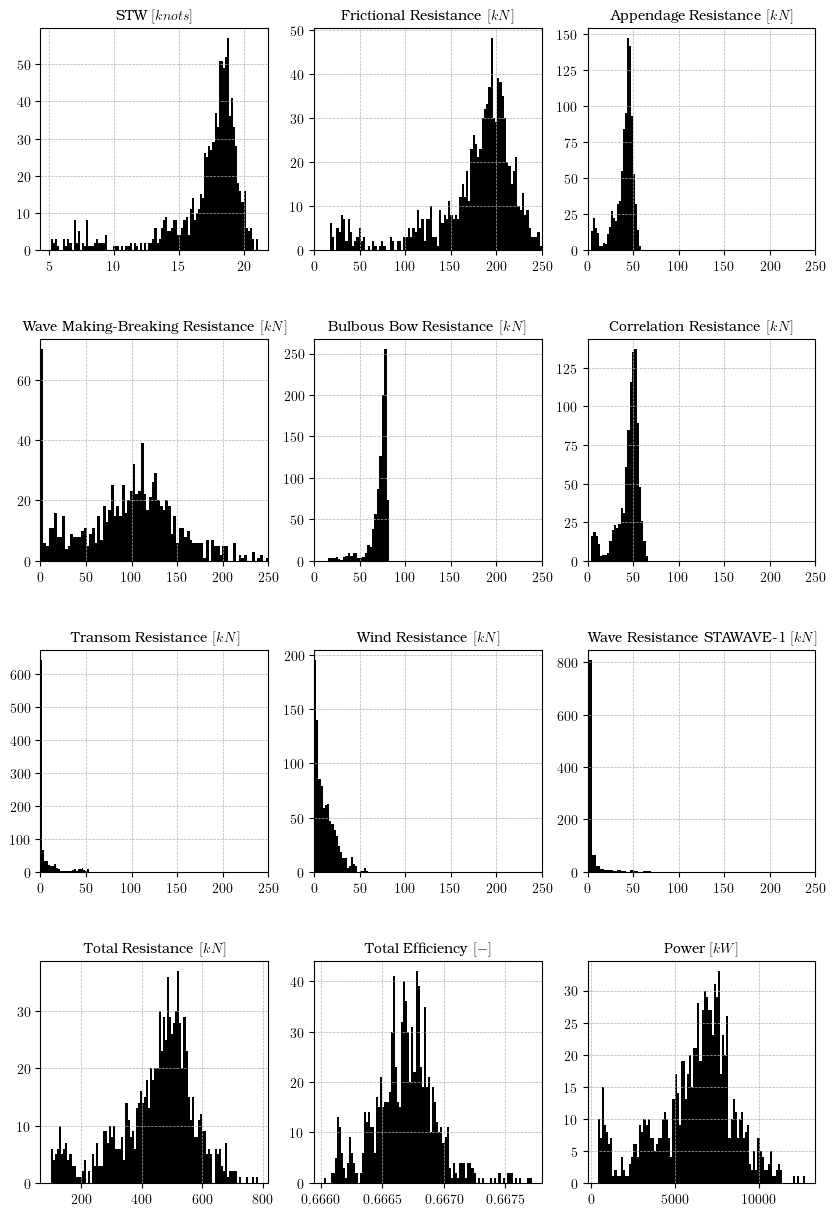
\includegraphics[width=.9\linewidth]{02_figures/resistance_power_hist.png}
    \caption{Histogram of encountered resistances for $DS_{year}$}
    \label{fig:hist_resistance_power_yr}
\end{figure}

For calm water resistance $R_{CALM}$, the largest portion is attributed to the frictional resistance $R_F$, which accounts for approximately $39\%$ of $R_{TOTAL}$ when considering the mean. Following this, the wave-making and breaking resistance $R_W$ contribute around $21\%$. Subsequently, the bulbous bow resistance $R_{B}$ accounts for approximately $16\%$, the correlation resistance $R_{A}$ around $10\%$, and the appendage resistance $R_{APP}$ at approximately $8\%$. The transom resistance $R_{TR}$ has a relatively negligible impact on $R_{CALM}$, accounting for only about $1\%$.\\

Regarding the added resistance due to surrounding weather conditions, the contribution of added resistance due to wind $R_{AA}$ are noticeable and adds a significant amount to the total resistance $R_{TOTAL}$. In contrast, the added resistance due to waves $R_{AW}$ is comparatively negligible. This behaviour can be explained by referring to \Cref{tbl:testyear_dataset_descriptive}, the sea conditions along the ship's sailing path are relatively calm, with a mean significant wave height $H_{1/3}$ of $0.77$ m and a mean wind speed of $6.45$ m/s. By only considering the mean, the combined additional resistance to weather conditions only makes up about $3.5\%$ of the total resistance.\\

These results further validate the BBM's ranking of ship draught $T$ as the most significant physical factor that affects the ship speed. The WBM also further confirm the BBM suggestion that wave resistance might have a more significant impact on the speed compared to wind resistance. This is evident from the maximum achievable resistance of $R_{AA}$ and $R_{AWL}$ shown in \Cref{tbl:PB_act_descriptive_yr}. However, over the journey, the mean of $R_{AWL}$ is significantly lower, primarily due to the condition in \Cref{eqn:stawave1}, which only consider the wave correction force within $\pm 45$° off bow.\\  

\begin{table}[h]
    \footnotesize
    \centering
    % \resizebox {\textwidth}{!}
    {\begin{tabular}{ p{0.04\linewidth} p{0.03\linewidth} c c c c c c c c }
    \hline
    Features && Count & Mean & std & Min & 25\% & 50\% & 75\% & Max \\
    \hline
    $STW$ & $[kt]$ & 957.00 &  17.03 &  3.10 &  5.14 &  16.62 &  18.07 &  18.79 &  21.08 \\
    $R_F $&$[kN]$ & 957.00 & 174.65 & 49.25 & 17.17 & 162.08 & 189.16 & 205.18 & 262.25 \\
    $R_{APP} $&$[kN]$ & 957.00 &  39.52 &  11.29 &  3.64 &  36.53 &  43.03 &  46.46 &  58.25 \\
    $R_{W} $&$[kN]$ & 957.00 &  96.51 &  55.49 &  0.00 &  61.08 & 102.36 & 129.98 & 297.53 \\
    $R_{B} $&$[kN]$& 957.00 &  71.23 &  11.30 & 15.59 &  69.79 &  74.93 &  77.64 &  82.20 \\
    $R_{TR} $&$ [kN]$ & 957.00 &   5.58 &  11.60 &  0.00 &   0.00 &   0.00 &   4.70 &  53.56 \\
    $R_{A} $&$ [kN]$ & 957.00 &  44.45 &  12.85 &  3.92 &  41.03 &  48.37 &  52.44 &  66.23 \\
    $R_{AA}$&$ [kN]$ & 957.00 &  12.15 &  11.27 &  0.01 &   3.07 &   8.74 &  18.08 &  59.50 \\
    $R_{AWL}$&$ [kN]$ & 957.00 &    3.48 &   11.23 &   0.00 &    0.00 &    0.00 &    1.17 &   116.18 \\
    $R_{TOT}$&$ [kN]$ & 957.00 &  447.57 &  129.17 & 100.29 &  387.05 &  473.26 &  527.77 &   784.72 \\
    $\eta_{TOT}$&$ [\%]$ & 957.00 &   0.67 &   0.00 &  0.67 &   0.67 &   0.67 &   0.67 &   0.67 \\
    $P_{B} $&$[kW]$ & 957.00 & 6173.34 & 2361.10 & 397.02 & 4987.21 & 6607.35 & 7654.90 & 12755.90 \\
    \hline
    \textbf{FOC}&$[T/h]$ & 957.00 &   1.04 &   0.40 &  0.06 &   0.84 &   1.11 &   1.29 &   2.09 \\
    \hline
    \end{tabular}}
\caption{Descriptive statistics of Power estimation method}\label{tbl:PB_act_descriptive_yr}
\end{table}

By considering the total resistance $R_{TOTAL}$ and the total efficiencies $\eta_{TOTAL}$, the brake power $P_B$ can be calculated. Using the brake power and the corresponding speeds, a power-to-speed curve can be plotted. This curve can then be transformed into a bunker-to-speed curve, which enables the estimation of the energy required for different operating speeds.\\ 

\begin{figure}[h!]
    \centering
    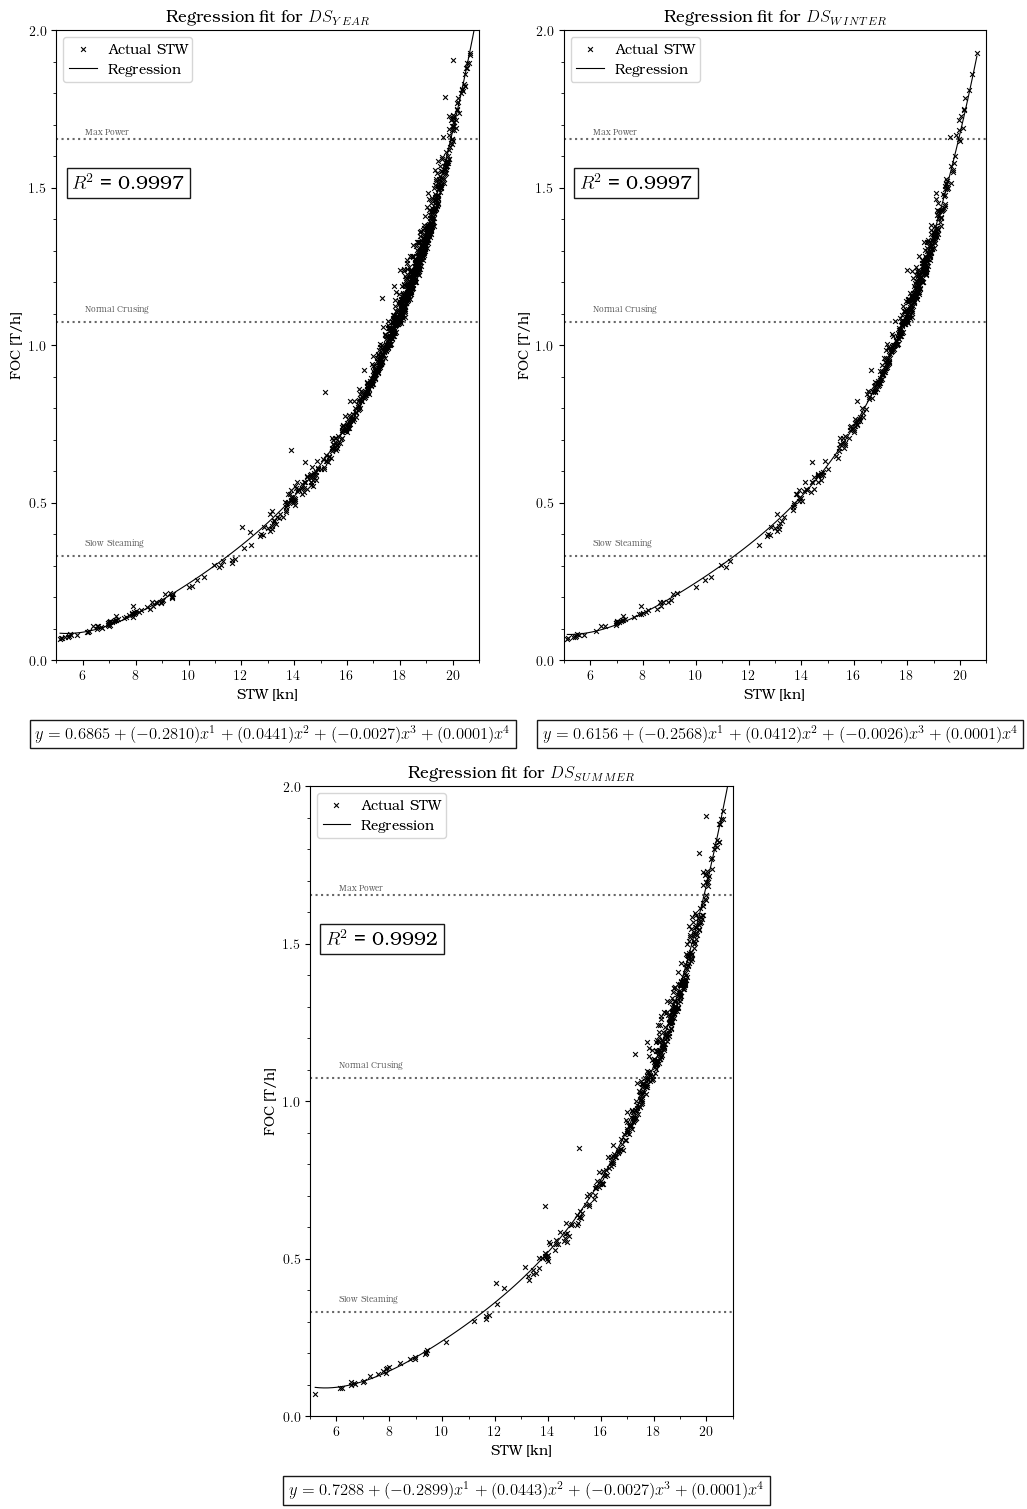
\includegraphics[width=.9\linewidth]{02_figures/poly_act_combi.png}
    \caption{Bunker-to-speed curve for actual data}
    \label{fig:FOC_plot_act_combi}
\end{figure}

To determine the most suitable regression fit, various polynomial regression lines with different orders are assessed. The selection of the optimal model is based on achieving the highest $R^2$ score while minimising the Mean Squared Error (MSE). To ensure robust model selection, the data from each dataset is partitioned into training and validation sets, allowing thorough validation of model performance. The evaluation of regression fits reveals that a polynomial regression of order $n=4$ is adequate to represent the relation between bunker consumption and STW. This model attains a $R^2$ score of approximately $99\%$ and significantly reduces the MSE compared to the $n=3$ model. Furthermore, as indicated in \Cref{tbl:polyfit_scores_errors}, there is no substantial performance enhancement when progressing from $n=4$ to $n=5$.\\

% \begin{table}[h]
%     \footnotesize
%     % \small
%     \centering
%     % \resizebox {\textwidth}{!}
%     {\begin{tabular}{ l c c c }
%     \hline
%     Dataset  & Polynomial Order & $R^2$ & MSE \\
%     & $n$ & [$\%$] & [$(T/h)^2] \cdot 10^{-3}$ \\ 
%     \hline
%     $DS_{year}$ & 1 & 86.95 & 20.62 \\
%      & 2 & 98.69 & 2.07 \\  
%      & 3 & 99.86 & 0.22 \\
%      & 4 & 99.96 & 0.06 \\
%      & 5 & 99.97 & 0.05 \\
%      $DS_{winter}$ & 1 & 87.64 & 21.41 \\
%      & 2 & 98.86 & 1.97 \\  
%      & 3 & 99.81 & 0.33 \\
%      & 4 & 99.95 & 0.08 \\
%      & 5 & 99.96 & 0.06 \\
%      $DS_{summer}$ & 1 & 86.53 & 27.67 \\
%      & 2 & 98.77 & 2.52 \\  
%      & 3 & 99.81 & 0.39 \\
%      & 4 & 99.93 & 0.15 \\
%      & 5 & 99.92 & 0.16 \\
%     \hline
%     \end{tabular}}
% \caption{Performance indices for FOC regression functions}\label{tbl:polyfit_scores_errors}
% \end{table}

\begin{table}[h]
    \footnotesize
    % \small
    \centering
    % \resizebox {\textwidth}{!}
    {\begin{tabular}{ l c c c c c c c }
    \hline
    Dataset & &  & \multicolumn{5}{c}{Polynomial Order}\\
    & Metric & Unit & 1 & 2 & 3 & 4 & 5 \\
    \hline
    $DS_{year}$ & $R^2$ & [$\%$] & 86.95 & 98.69 & 99.86 & 99.96 & 99.97 \\
    &MSE & [$(T/h)^2] \cdot 10^{-3}$ & 20.62 & 2.07 & 0.22 & 0.06 & 0.05 \\   
    $DS_{winter}$ & $R^2$ & [$\%$] & 87.64 & 98.86 & 99.81 & 99.95 & 99.96 \\
    &MSE & [$(T/h)^2] \cdot 10^{-3}$ & 21.41 & 1.97 & 0.33 & 0.08 & 0.06\\
    $DS_{summer}$ & $R^2$ & [$\%$] & 86.53 & 98.77 & 99.81 & 99.93 & 99.92\\
    &MSE & [$(T/h)^2] \cdot 10^{-3}$ & 27.67 & 2.52 & 0.39 & 0.15 & 0.16\\

    % & $n$ & [$\%$] & [$(T/h)^2] \cdot 10^{-3}$ \\ 
    % $DS_{year}$ & 1 & 86.95 & 20.62 & $R^2$ & MSE \\
    %  & 2 & 98.69 & 2.07 \\  
    %  & 3 & 99.86 & 0.22 \\
    %  & 4 & 99.96 & 0.06 \\
    %  & 5 & 99.97 & 0.05 \\
    %  $DS_{winter}$ & 1 & 87.64 & 21.41 \\
    %  & 2 & 98.86 & 1.97 \\  
    %  & 3 & 99.81 & 0.33 \\
    %  & 4 & 99.95 & 0.08 \\
    %  & 5 & 99.96 & 0.06 \\
    %  $DS_{summer}$ & 1 & 86.53 & 27.67 \\
    %  & 2 & 98.77 & 2.52 \\  
    %  & 3 & 99.81 & 0.39 \\
    %  & 4 & 99.93 & 0.15 \\
    %  & 5 &   & 0.16 \\
    \hline
    \end{tabular}}
\caption{Performance indices for FOC regression functions}\label{tbl:polyfit_scores_errors}
\end{table}

The resulting bunker-to-speed curve plots are shown in figure \Cref{fig:FOC_plot_act_combi}, The resulting functions align with the findings from \bcitet{Psaraftis.2013}. The cubic law dictates that the fuel consumption rate can be defined with a proportional factor and sailing speed raised to the power of $\alpha = 3$ \bcitep{Du.2019}. However, \bcitet{Psaraftis.2013} stated that the cubic law is not applicable for low speeds, and the factor $\alpha$ can be 4 or 5 or possibly even higher for some types of ships or when travelling at high speeds.\\ 

\pagebreak

However, the observations outlined in \Cref{tbl:polyfit_scores_errors} imply that the cubic law may still be applicable within the context of this case study. The slight improvement in function fit performance from $n = 3$ to $n = 4$ is not substantial. There is no notable reduction in the MSE, and the achieved $R^2$ score for $n = 3$ exhibits minor variation from the best-fit model. Given that the model is primarily intended to characterize ship journeys at a steady sailing state, the limitations of the cubic law highlighted by \citet{Psaraftis.2013} may not be directly applicable.\\

% \begin{figure}[h!]
%     \centering
%     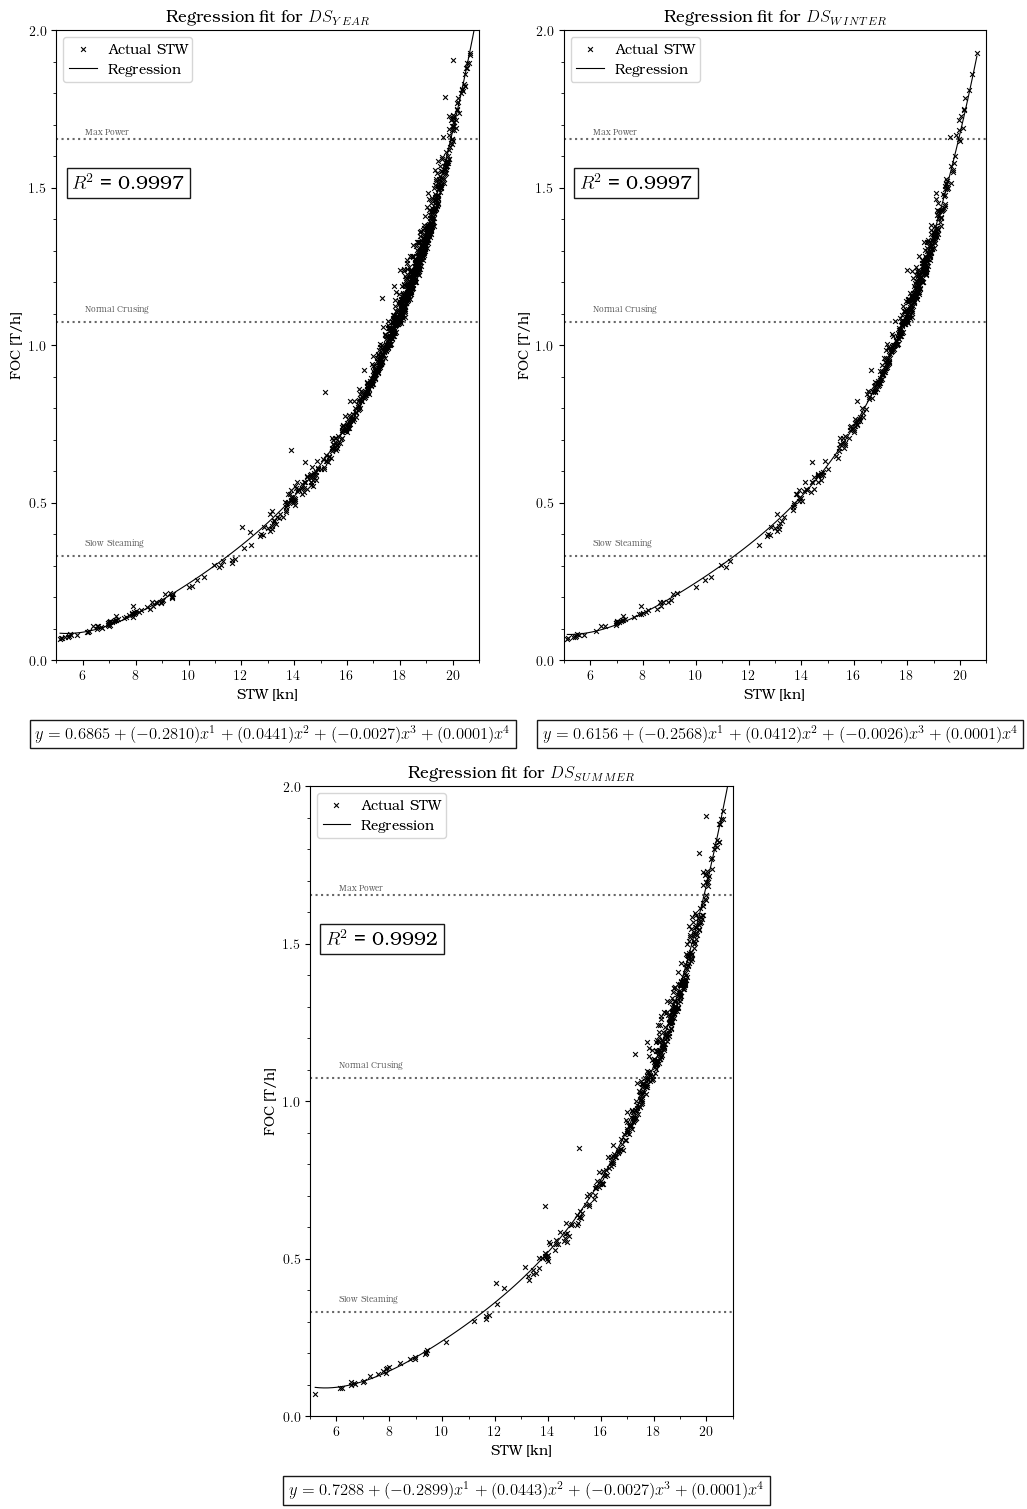
\includegraphics[width=.9\linewidth]{02_figures/poly_act_combi.png}
%     \caption{Bunker-to-speed curve for actual data}
%     \label{fig:FOC_plot_act_combi}
% \end{figure}

The results also reveal instances where the model predicts ship speeds exceeding the maximum engine rating, which is physically impossible. This issue can be attributed to the conversion of SOG to STW. Analysing openly accessible data from the study conducted by \bcitet{JoanPeturPetersen.2011}\footnote{\url{http://cogsys.imm.dtu.dk/propulsionmodelling/}}, a noticeable distinction between SOG and STW can be observed, typically differing by a factor of approximately 0.85. In the context of this case study, even after accounting for the current correction, the difference in speeds remains marginal. This suggests that the conversion of SOG to STW should also include the influence of speed reduction due to wind and waves. \bcitet{Molland.2017} presented illustrative speed loss curves based on varying Beaufort scales, as illustrated in Figure \Cref{fig:molland17_speedloss_windwave}. Furthermore, \bcitet{Molland.2017} presented two direct speed loss formulae due to wind and wave effects by \bcitet{Aertssen.1975} and \bcitet{kwon.2008}. However, these formulae possess a limited range of applicability and are not optimised for different vessel types. Therefore, these formulae are not implemented in this thesis.\\

\begin{figure}[ht]
    \centering
    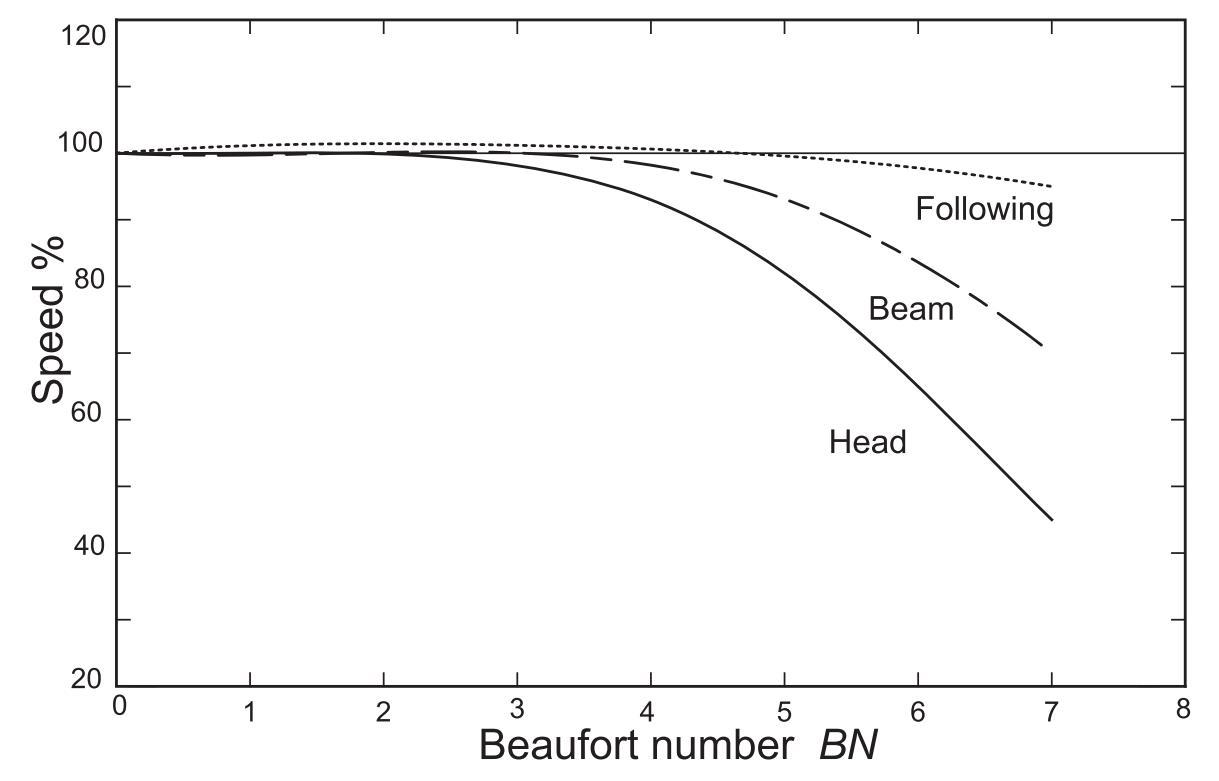
\includegraphics[width=.7\linewidth]{02_figures/molland17_speedlosscurve.jpg}
    \caption{Speed loss with increase in Beaufort Number BN \bcitep{Molland.2017}}
    \label{fig:molland17_speedloss_windwave}
\end{figure}

\subsection{Result and Discussion of WBM on predicted SOG}\label{sec:WBM_result_discussion}

Table \Cref{tbl:FOC_scores_errors} presents the results for FOC prediction across different modelling approaches and datasets. The ETR model demonstrated the best predictive performance, it is closely trailed by RFR and the followed by DTR. The similarity in results can be attributed to the sequential nature of the GBM approach. Notably, there is a decline in the $R^2$ score, explained variance, and MAPE across all models. This decrease in performance could be attributed to the inherent nonlinearity of the WBM, which tends to amplify FOC prediction errors at higher ship speeds. This phenomenon is exemplified by the case study conducted by \bcitet{Birk.2019}, as depicted in Figure \Cref{fig:birk19_Pb_nonlinear}. In this study, a discrepancy of $1$ knot in ship speed resulted in a power difference of around $1200$ kW at lower speeds. However, at higher speeds, the power difference escalated to about $2300$ kW. Assuming an identical SFOC for the engine in both the \bcitet{Birk.2019} case study and this thesis, this discrepancy translates to FOC differences of approximately $0.2$ T/h and $0.4$ T/h, respectively.

\begin{table}[h]
    \footnotesize
    % \small
    \centering
    % \resizebox {\textwidth}{!}
    {\begin{tabular}{ l l c c c c c c }
    \hline
    Model & Dataset & $R^2$ & expVar & MAE & RMSE & MAD & MAPE \\
    & & [$\%$] & [$\%$] & [$T/h$] & [$T/h$] & [$T/h$] & [$\%$]  \\ 
    \hline
    $\text{DTR}_{OPT}$ & $DS_{year}$ & 76.59 & 76.63 & 0.133 & 0.193  & 0.087 & 15.79  \\
    & $DS_{winter}$ & 78.24 & 78.25 & 0.123 & 0.179 & 0.080 & 15.38 \\
    & $DS_{summer}$ & 74.42 & 74.73 & 0.145 &  0.208 & 0.096 & 16.25 \\
    $\text{RFR}_{OPT}$ & $DS_{year}$  & 81.82 & 81.89 & 0.117 & 0.170 & 0.079 & 13.65 \\
    & $DS_{winter}$ & 86.55 & 86.56 & 0.099 & 0.141 & 0.069 & 12.08 \\
    & $DS_{summer}$ & 76.81 & 77.20 & 0.137 & 0.198 & 0.088 & 15.37 \\
    $\text{ETR}_{OPT}$ & $DS_{year}$ & 83.84 & 84.01 & 0.111 & 0.161 & 0.076 & 12.45\\
    & $DS_{winter}$ & \textbf{87.57} & \textbf{87.57} & \textbf{0.097} & \textbf{0.135} & \textbf{0.068} & \textbf{11.37} \\
    & $DS_{summer}$ & 79.86 & 80.49 & 0.127 & 0.184 & 0.082 & 13.64 \\
    MLR & $DS_{year}$ & 29.34 & 32.03 & 0.223 & 0.336 & 0.171 & 29.35 \\
    & $DS_{winter}$ & 11.98 & 13.09 & 0.212 & 0.360 &0.162& 33.02 \\
    & $DS_{summer}$ & 44.28 & 49.44 & 0.235 & 0.307 & 0.191 & 25.29 \\
    \hline
    \end{tabular}}
\caption{Performance indices for FOC prediction}\label{tbl:FOC_scores_errors}
\end{table}

\begin{figure}[ht]
    \centering
    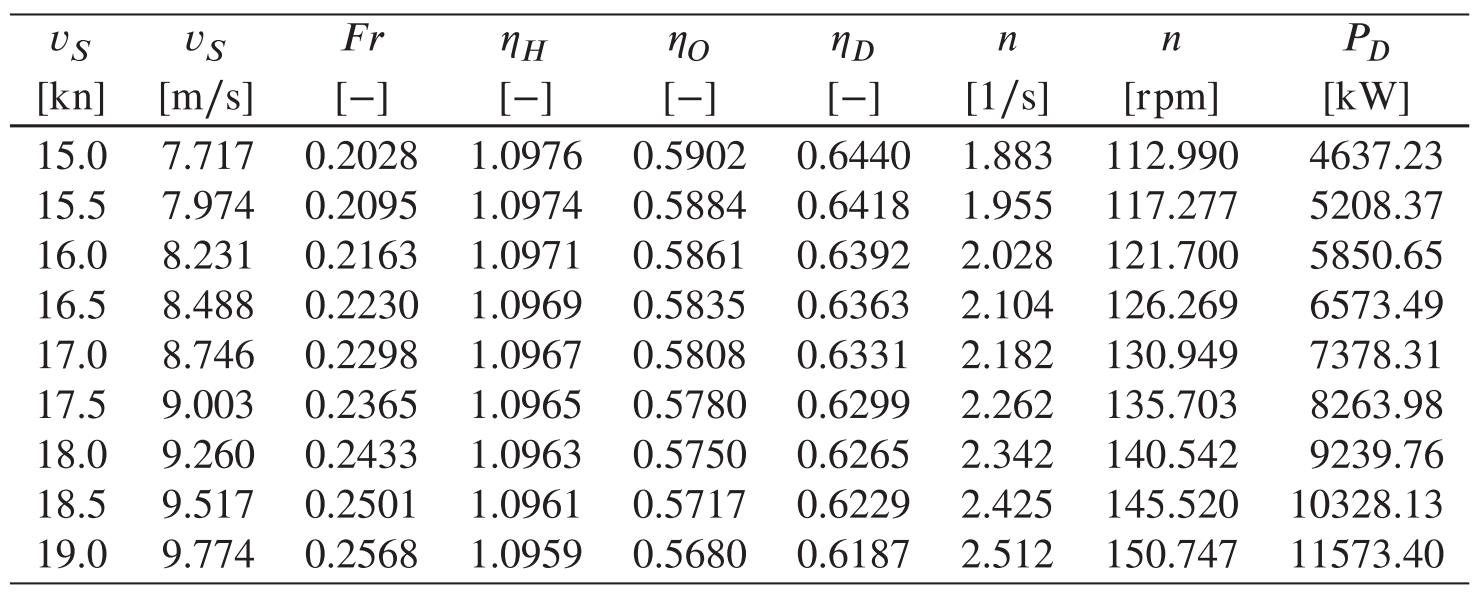
\includegraphics[width=.8\linewidth]{02_figures/birk19_Pb_nonlinear_case.jpg}
    \caption{Case study for power estimation by \bcitet{Birk.2019}}
    \label{fig:birk19_Pb_nonlinear}
\end{figure}

This phenomenon could also account for the model's limitations in accurately predicting FOC at higher end of STW, as indicated by the plot in Figure \Cref{fig:foc_act_all_yr}. The plots also demonstrated the underfitting behaviour of the models, \Cref{fig:foc_act_all_yr} shows that all models underpredict the FOC for STW higher than 20 knots. However, the model's prediction errors remain reasonable. For instance, considering the $DS_{year}$ dataset, the MAE ranges between $0.111$ T/h and $0.133$ T/h, in the context of a mean FOC of $1.04$ T/h.\\

The resulting bunker-to-speed curves for different models are illustrated in Figure \Cref{fig:FOC_plot_etr_combi} for ETR, \Cref{fig:FOC_plot_rfr_combi} for RFR, and \Cref{fig:FOC_plot_dtr_combi} for DTR. Overall, the plot for ETR exhibits the highest $R^2$ score. Nevertheless, the disparities are minimal, given that the functions are almost indistinguishable across different models.\\

% \begin{figure}
%     \centering
%     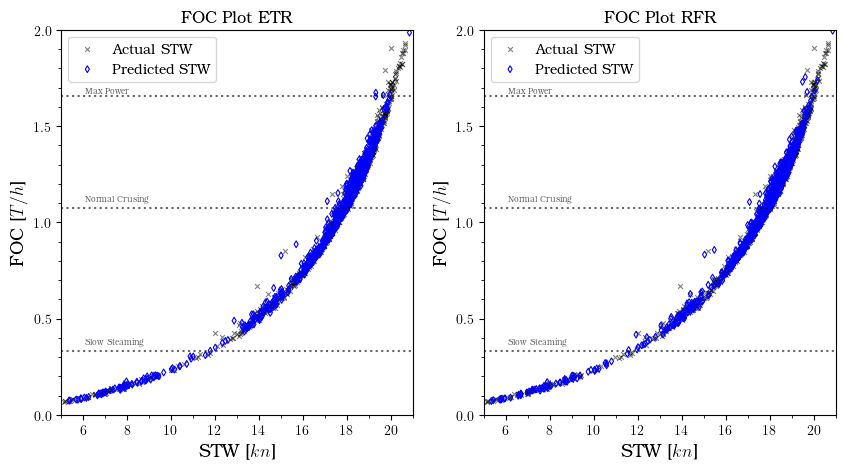
\includegraphics[width=.9\linewidth]{02_figures/FOC_act_pred_etr_rfr.png}
%     \caption{Predicted and Actual FOC for ETR and RFR using $DS_{year}$}
%     \label{fig:foc_etr_rfr_yr}
% \end{figure}

\begin{figure}
    \centering
    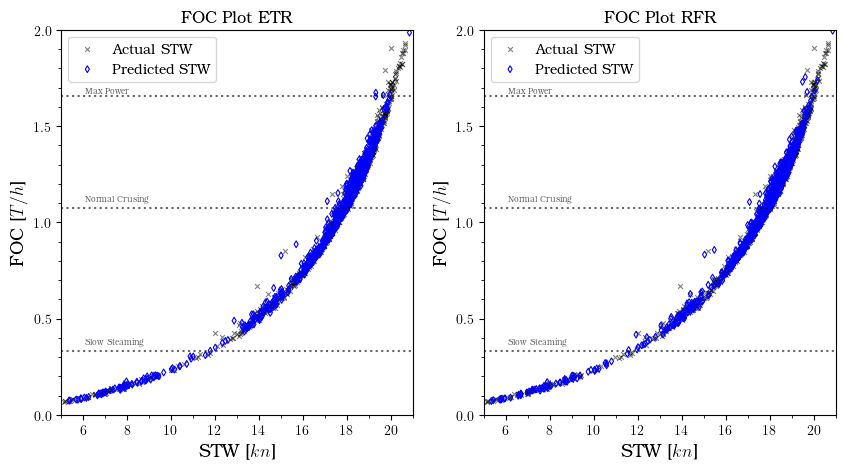
\includegraphics[width=.9\linewidth]{02_figures/FOC_act_pred_etr_rfr.png}\\
    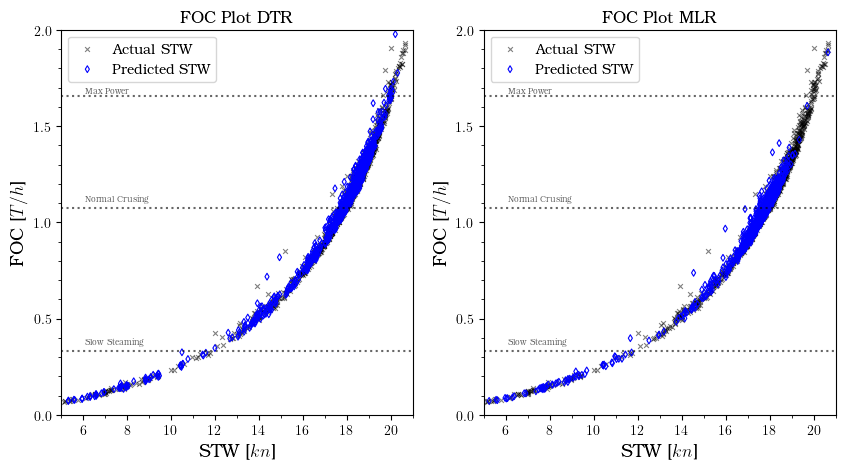
\includegraphics[width=.9\linewidth]{02_figures/FOC_act_pred_dtr_mlr.png}
    \caption{Predicted and Actual FOC for different models using $DS_{year}$}
    \label{fig:foc_act_all_yr}
\end{figure}

% \begin{figure}
%     \centering
%     \begin{minipage}[t]{0.5\textwidth}
%         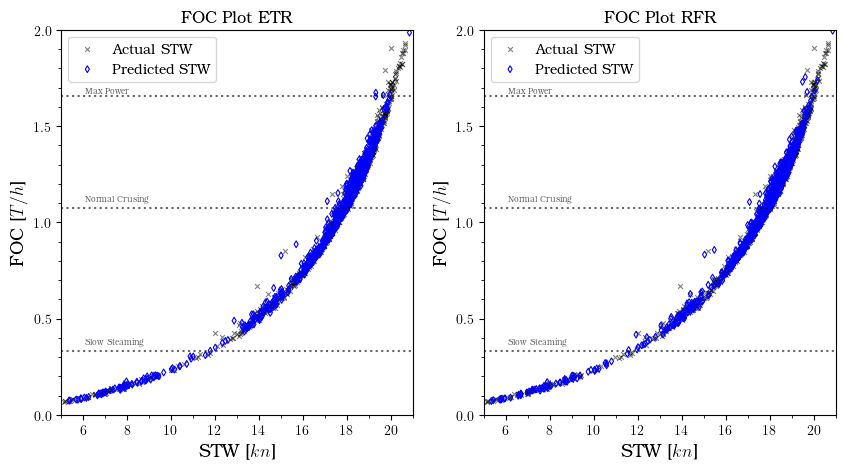
\includegraphics[width=\textwidth]{02_figures/FOC_act_pred_etr_rfr.png}
%         \caption{Caption for Image 1}
%         \label{fig:image1}
%     \end{minipage}%
%     \begin{minipage}[t]{0.5\textwidth}
%         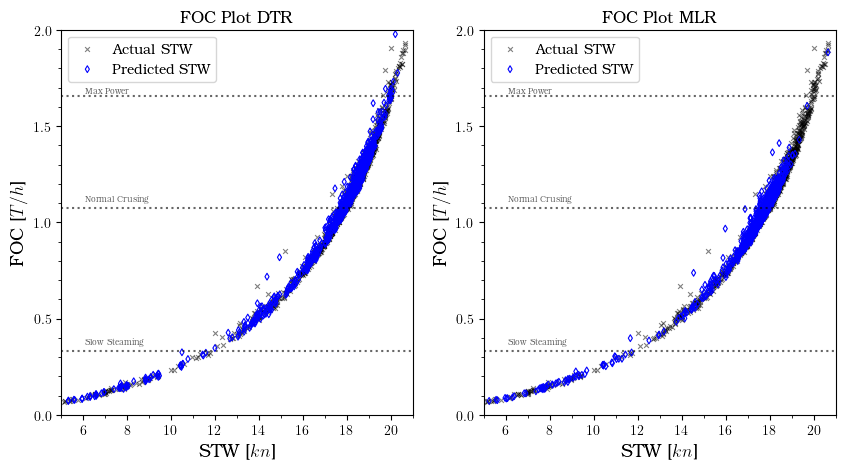
\includegraphics[width=\textwidth]{02_figures/FOC_act_pred_dtr_mlr.png}
%         \caption{Caption for Image 2}
%         \label{fig:image2}
%     \end{minipage}
%     \caption{Overall Caption for Both Images}
%     \label{fig:two_images}
% \end{figure}

\newpage

\begin{figure}[h!]
    \centering
    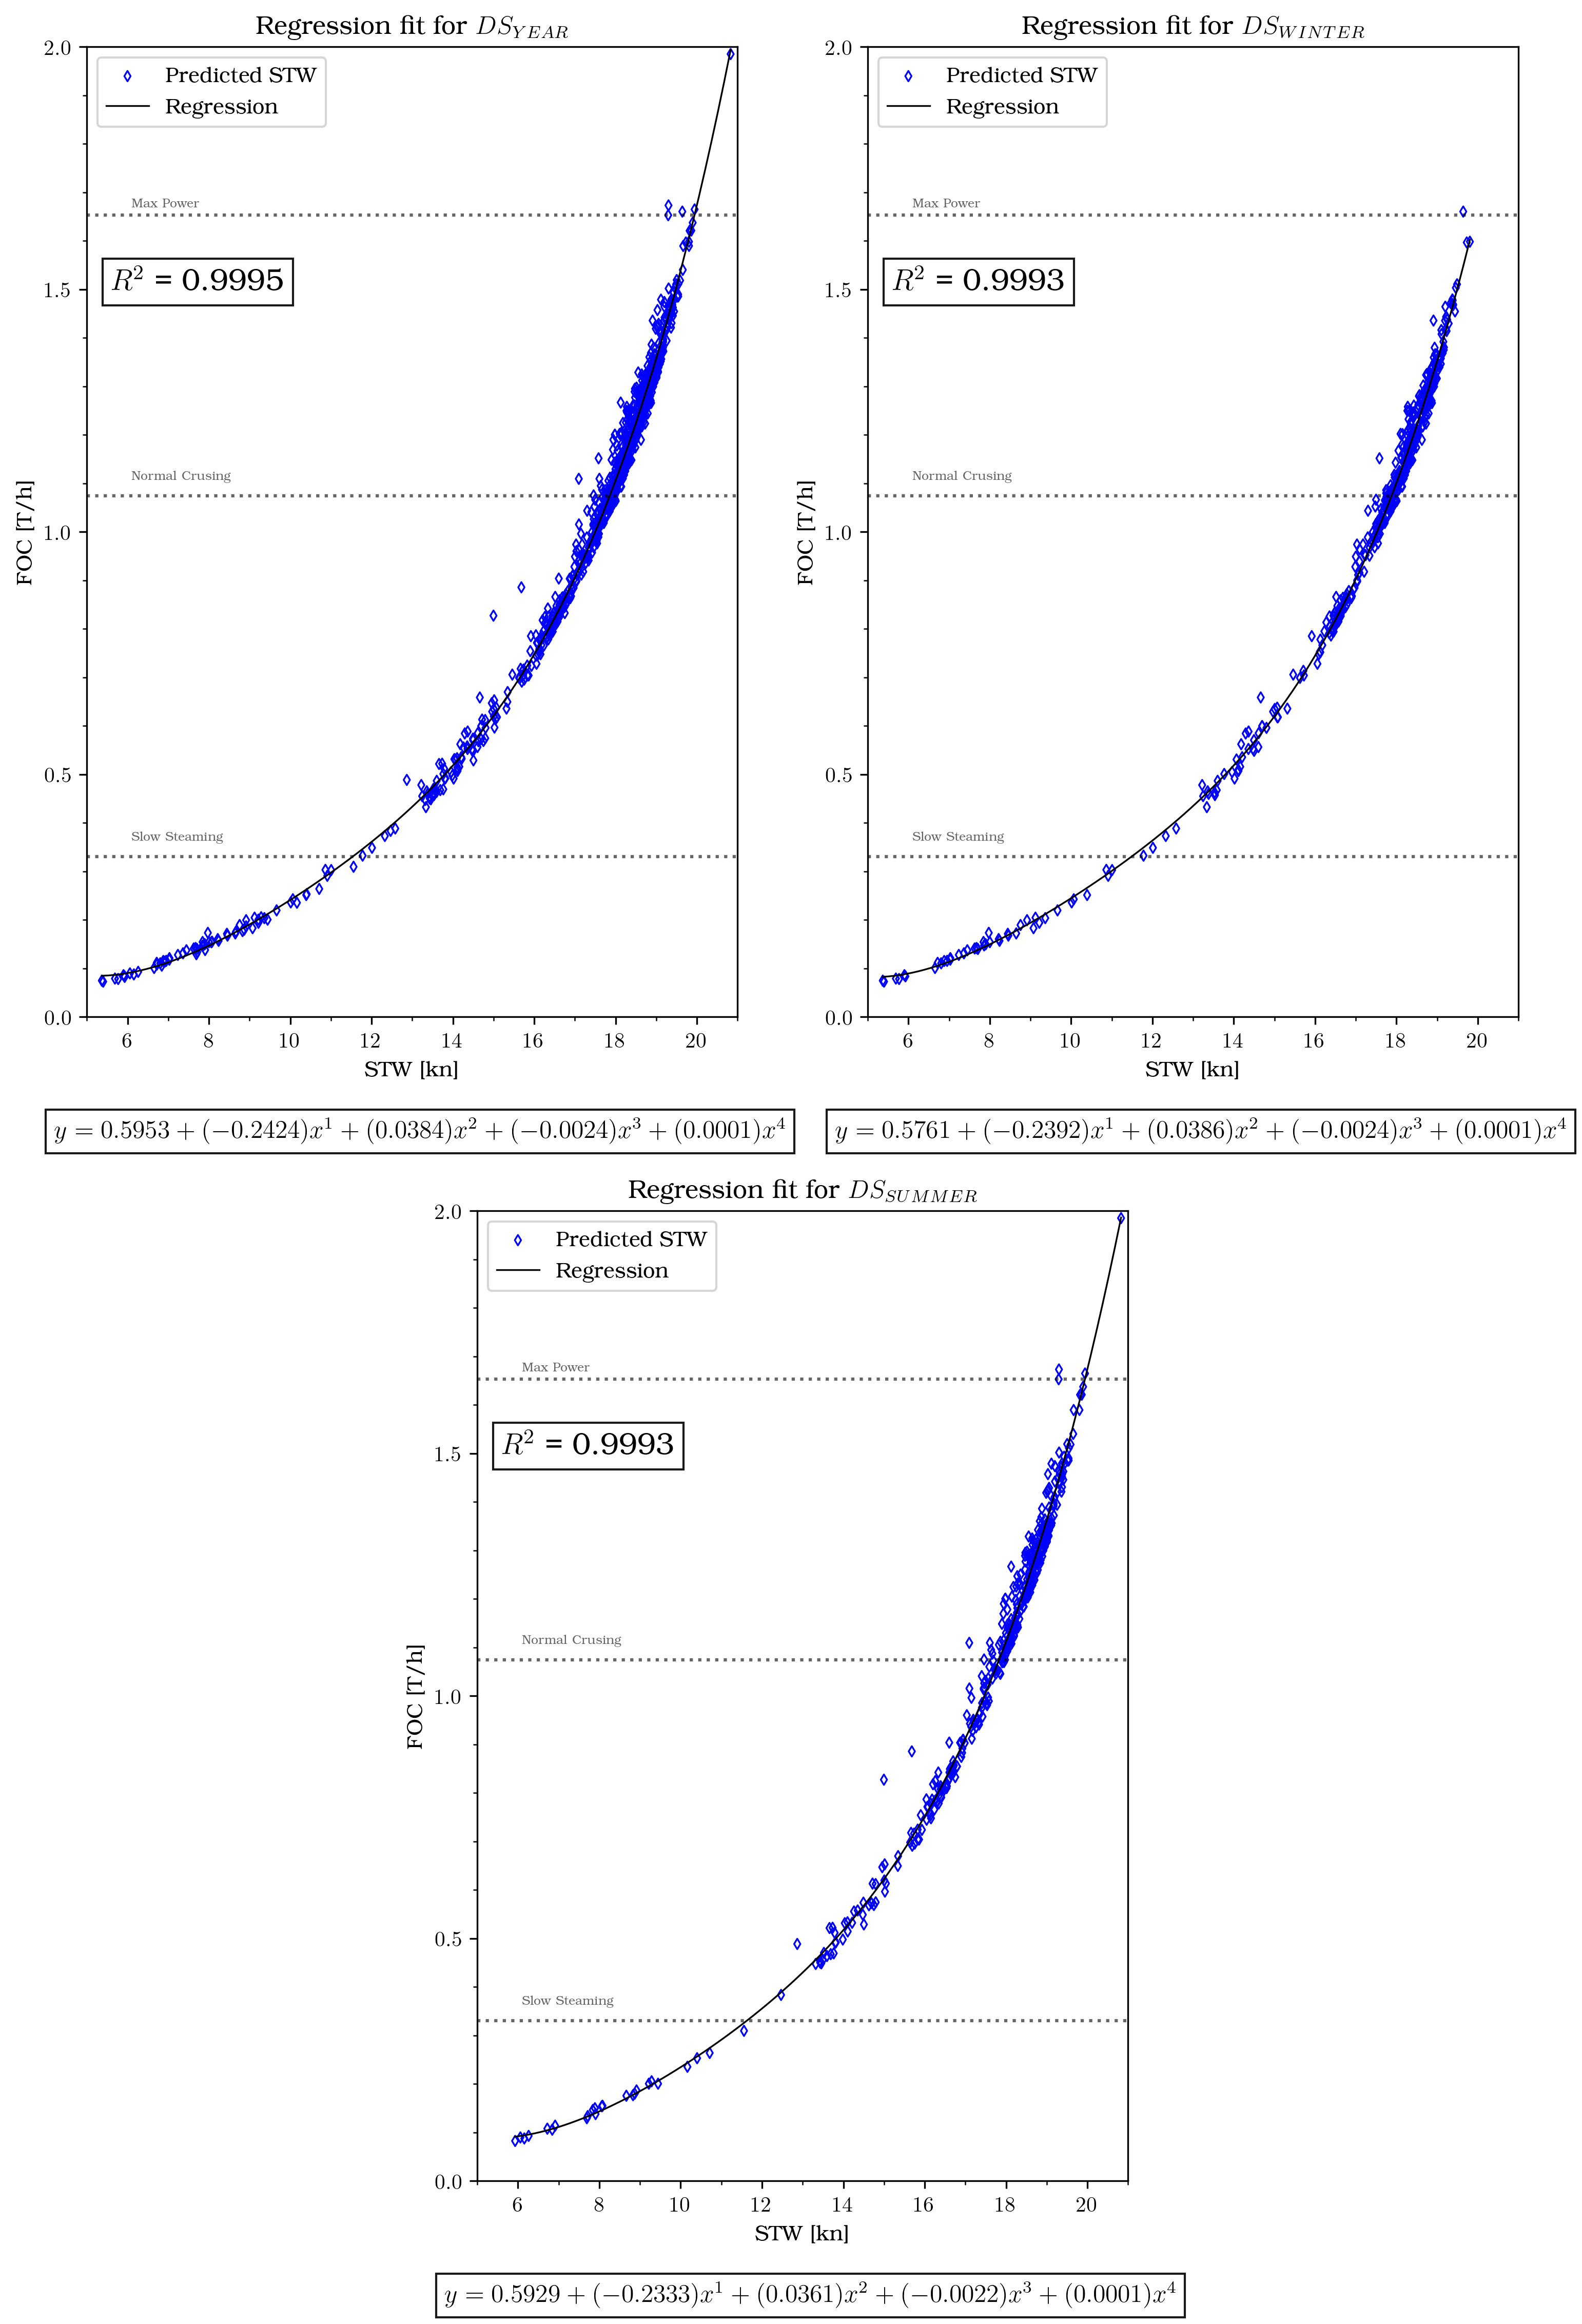
\includegraphics[width=.9\linewidth]{02_figures/poly_etr_combi.png}
    \caption{Bunker-to-speed curves generated from ETR}
    \label{fig:FOC_plot_etr_combi}
\end{figure}

\newpage

\begin{figure}[h!]
    \centering
    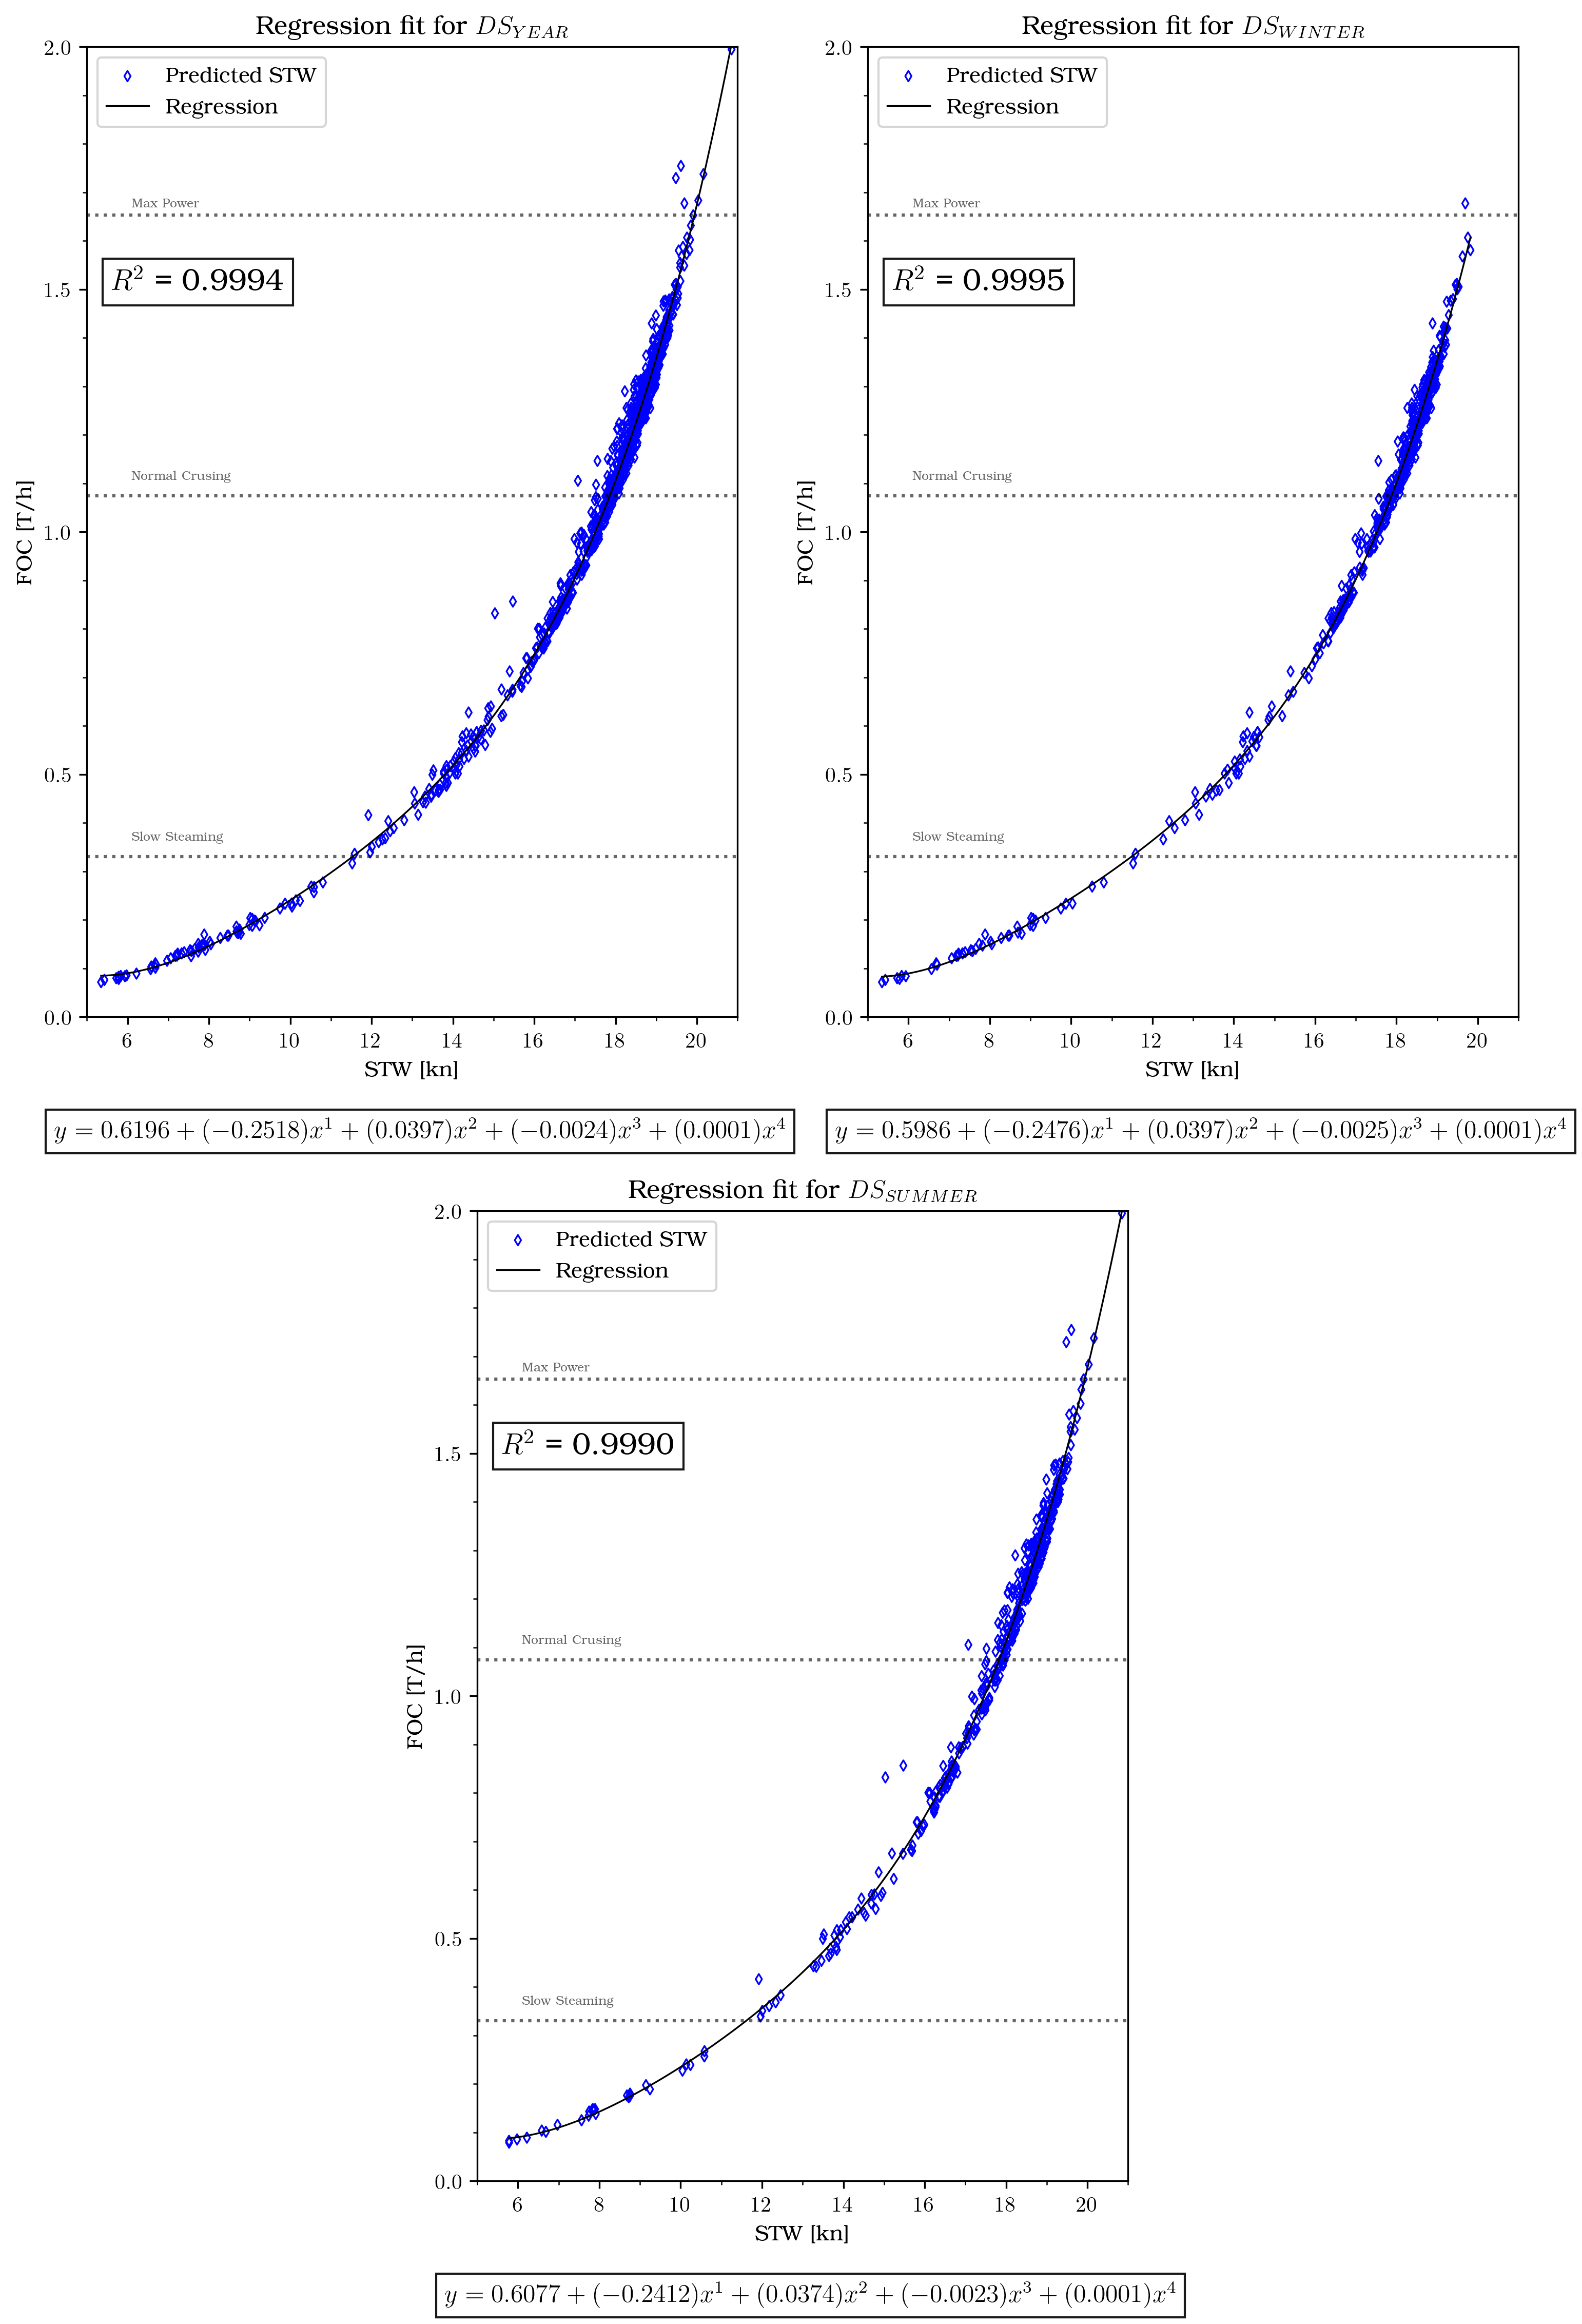
\includegraphics[width=.9\linewidth]{02_figures/poly_rfr_combi.png}
    \caption{Bunker-to-speed curves generated from RFR}
    \label{fig:FOC_plot_rfr_combi}
\end{figure}

\newpage

\begin{figure}[h!]
    \centering
    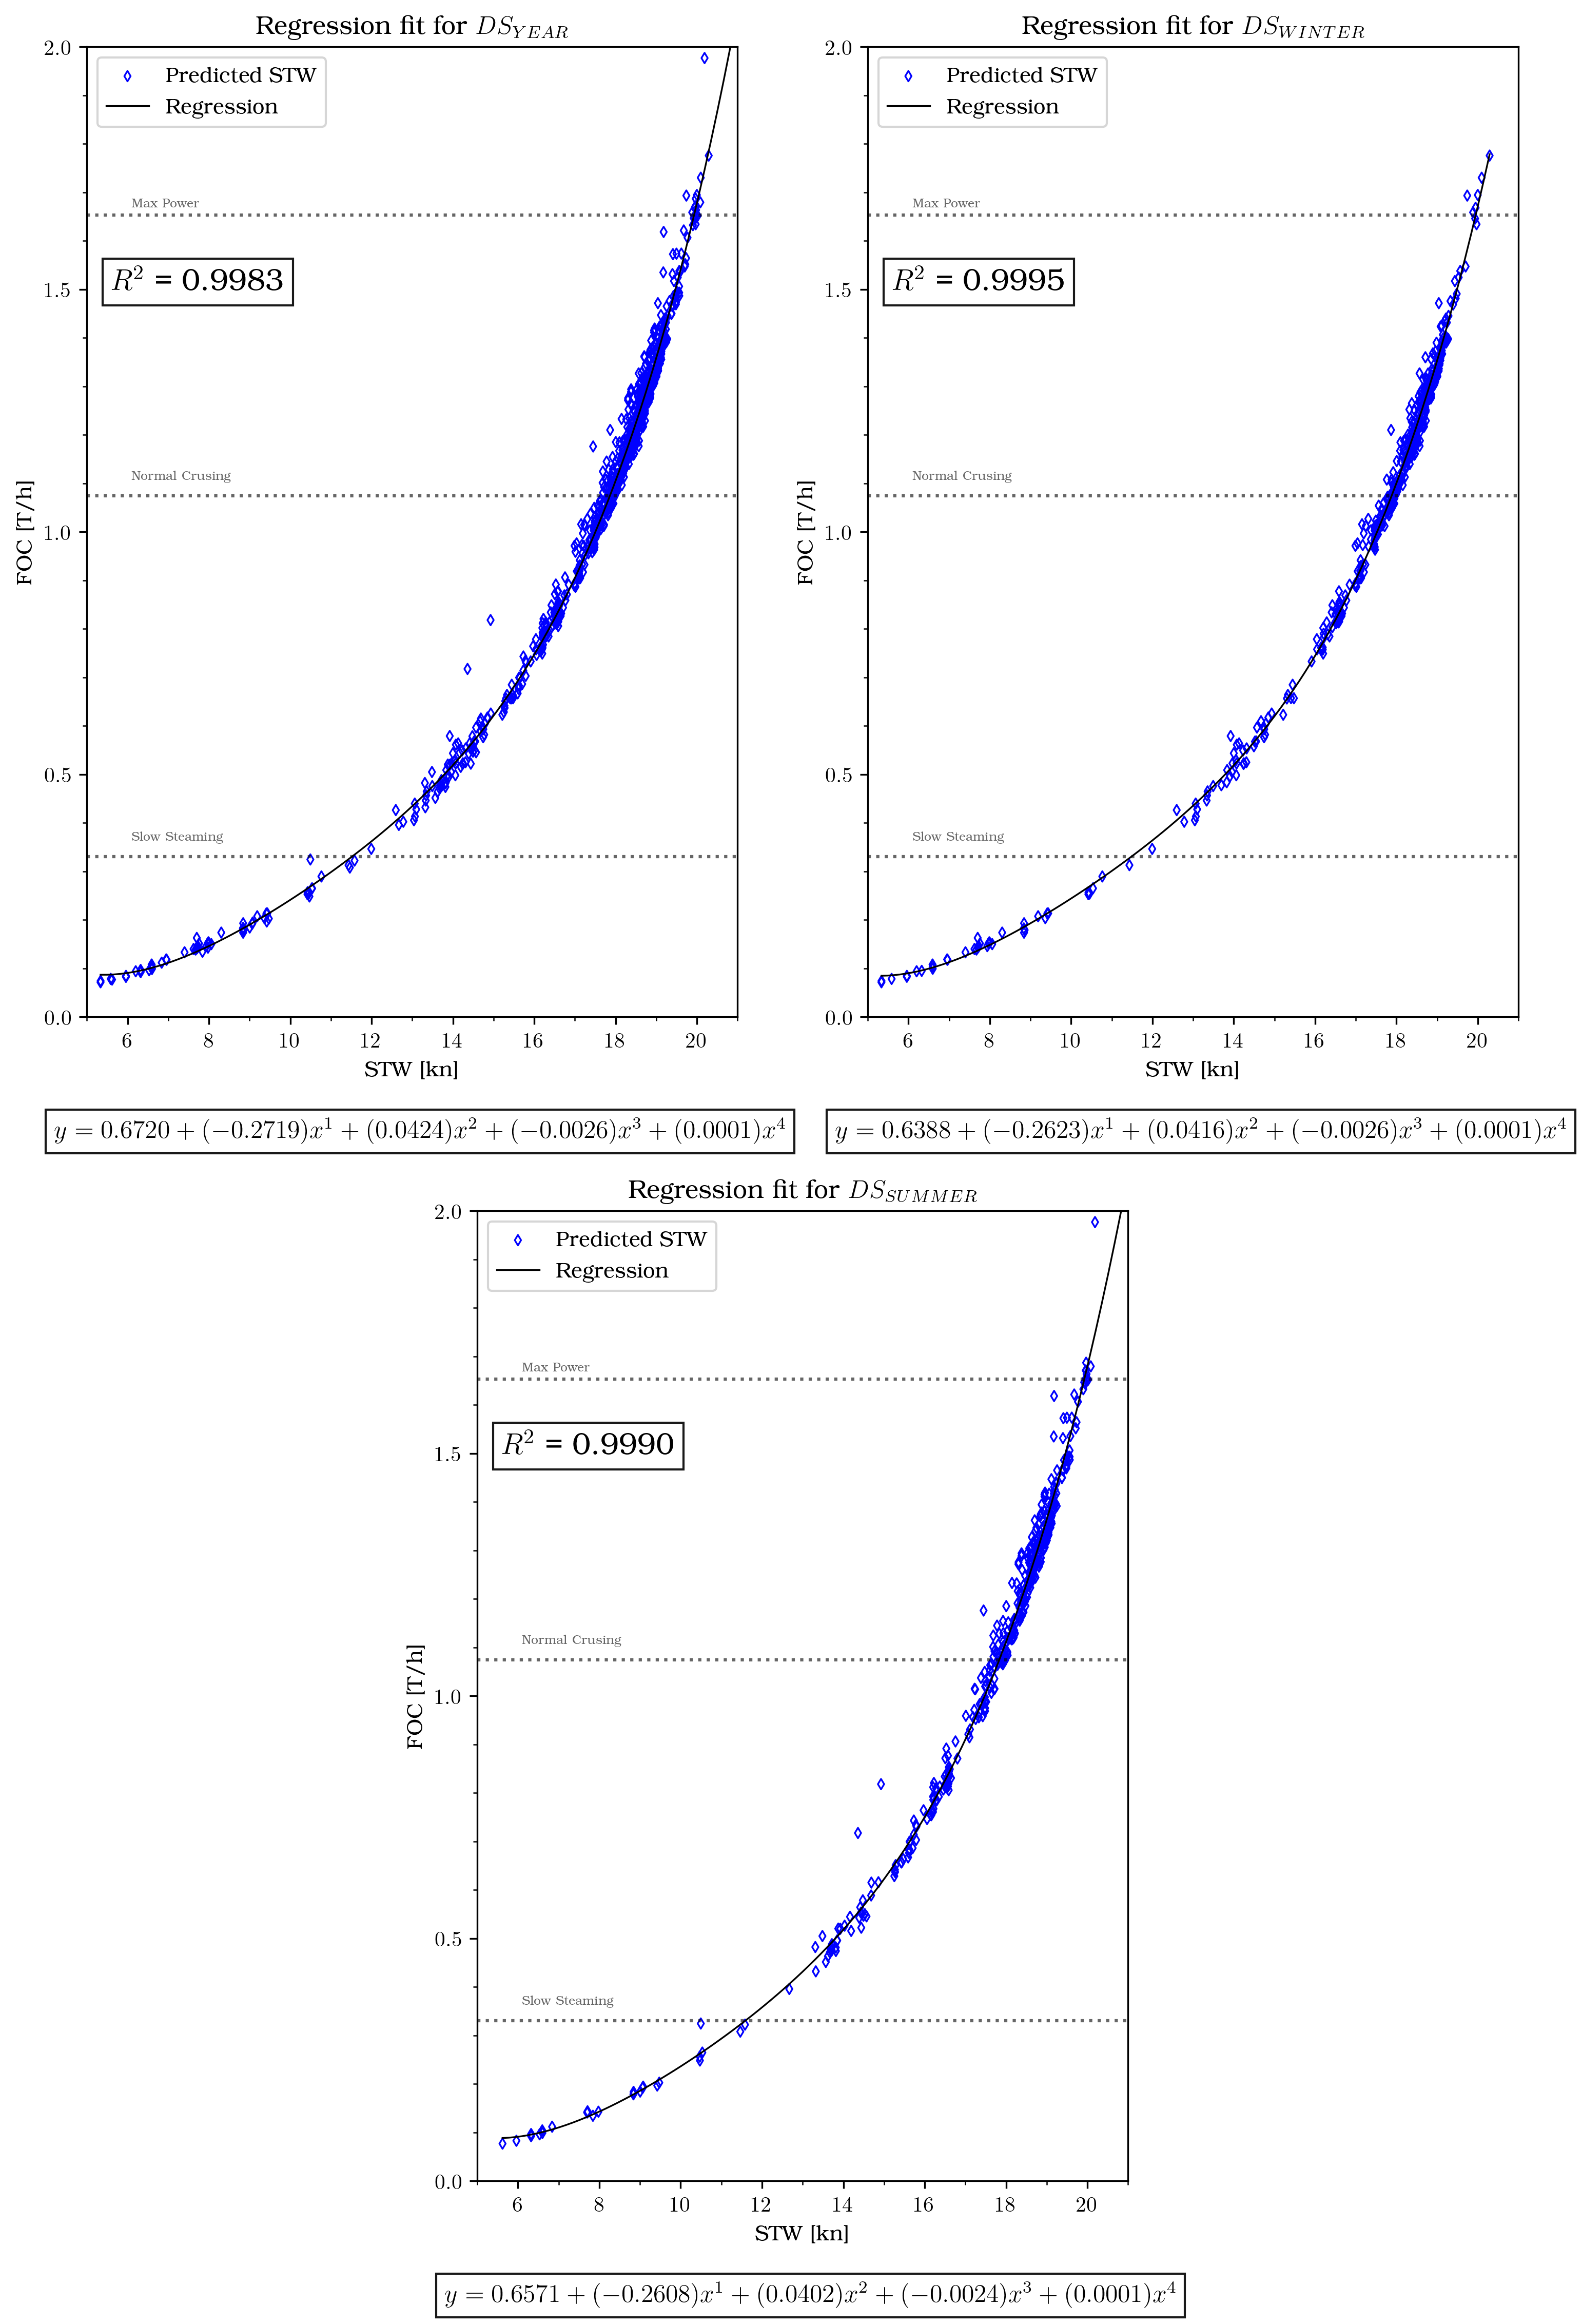
\includegraphics[width=.9\linewidth]{02_figures/poly_dtr_combi.png}
    \caption{Bunker-to-speed curves generated from DTR}
    \label{fig:FOC_plot_dtr_combi}
\end{figure}
\newpage

\subsection{Key Findings}\label{sec:key_findings}

\subsubsection*{\emph{Performance of BBM}}

The best predictive performance for SOG from different datasets was obtained by ETR, which is able to achieve $R^2$ score of $95\%$ and MAE of 0.53 knots. The performance gap between RFR and ETR is slight, RFR is able to obtain $R^2$ score of $93\%$ and MAE of 0.55 knots. Despite being a relatively simpler model to both RFR and ETR, DTR performs reasonably well for SOG and FOC prediction, it obtained a $R^2$ score of $89\%$ and MAE of 0.69 knots. A simple MLR model may be insufficient for implementation, as substantial performance gap is found between MLR and other tree-based models, with $R^2$ score of $72\%$ and MAE of 1.16 knots.\\

The quality and quantity of data are closely interrelated factors that significantly impact model performance. There are noticeable differences in the performance between the $DS_{winter}$ and $DS_{summer}$ datasets, with an increase of approximately $6\%$ in the $R^2$ score and a reduction of about 0.1 knots in MAE is achievable with an increase in about 50 data points. However, the quantity of data alone is insufficient to ensure an increase in model performance. This observation is evident from the $DS_{year}$ datasets, which contain approximately twice as much data as the other datasets, yet the model's performance is not superior to that of the $DS_{winter}$ dataset. This suggests that the quality of the $DS_{summer}$ dataset may compromise the model's performance when using the $DS_{year}$ dataset.\\

For BBM, hyperparameter optimisation substantially benefits the DTR model, while the impact of optimization on RFR and ETR models is minimal. Analysing feature importances and model structure visualisation, the RFR model recognizes draught as the most influential factor affecting SOG prediction. While the ETR and DTR models also identify this factor, but with a lesser degree of recognition.\\

\subsubsection*{\emph{Performance of WBM}}


Due to the sequential approach of GBM, the predictive performance of BBM is carried over to WBM during FOC prediction. Similar to BBM, ETR achieved a $R^2$ score of $88\%$ with MAE of 0.097 T/h for the best dataset. This is then followed by RFR which achieved a $R^2$ score of $87\%$ and MAE of 0.099 T/h, DTR obtained $78\%$ for $R^2$ and 0.123 T/h for MAE. MLR sees a very significant decline in $R^2$ score, only achieving $44.28\%$ and MAE of 0.34 T/h.\\

The nonlinear relation between speed and bunker means that significant deviation of SOG leads to an amplified magnitude of errors for FOC. This is evident in the case of MLR, the model already made relatively larger errors than other tree-based models during SOG prediction. With that, it is important to ensure that the SOG prediction of BBM is to be optimised as much as possible to ensure accurate FOC prediction. In the case study, the decline in performance is apparent when comparing the SOG prediction in \Cref{tbl:SOG_pred_descriptive} and \Cref{tbl:FOC_scores_errors}.\\

The power estimation method by Holtrop-Mennen method resulted in a 4\textsuperscript{th} order bunker-to-speed function. However, the resulting regression function of 3\textsuperscript{rd} order shows comparable performance. Therefore, a relatively simpler model such as cubic law is a feasible replacement for the WBM part of the GBM. For calm water resistance $R_{CALM}$, all resistance components make noticeable contributions to calm water resistance $R_{CALM}$ and the additional resistance due to wind and wave makes up about $3.5\%$ of total resistance $R_{TOT}$.\\

\subsubsection*{\emph{Application of outlier rejection to test data}}

Two possible solutions to improve model performance was presented \Cref{sec:result_discussion_BBM}, since the addition of data points is not feasible, the application of outlier rejection is adopted in this section. The outlier in higher speed is not applicable, however, for the lower limit, it was found to be around 8 knots which are based on the mean and standard deviation of $DS_{year}$ shown in \Cref{tbl:testyear_dataset_descriptive}. Due to the sparsity of data points at low SOG, the amount of data points is not compromised.\\
\begin{table}[h!]
    % \footnotesize
    \small
    \centering
    % \resizebox {\textwidth}{!}
    {\begin{tabular}{ l l c c c c c c }
    \hline
    Model & Dataset & $R^2$ & expVar & MAE & RMSE & MAD & MAPE \\
    & & [$\%$] & [$\%$] & [$kn$] & [$kn$] & [$kn$] & [$\%$]  \\ 
    \hline
    $\text{DTR}_{OPT}$ & $DS_{year}$ & 79.54 & 79.55 & 0.658 & 0.971 & 0.462 & 3.99 \\
    & $DS_{winter}$ & 84.17 & 84.17 & 0.584 & 0.847 & 0.407 & 3.53 \\
    & $DS_{summer}$ & 74.26 & 74.36 & 0.742  & 1.096 & 0.524 & 4.51 \\
    $\text{RFR}_{OPT}$ & $DS_{year}$  & 91.97 & 91.98 & 0.349 & 0.608 & 0.208  & 2.12 \\
    & $DS_{winter}$ & 95.35 & 95.35 & 0.303 & 0.459 & 0.201 & 1.83 \\
    & $DS_{summer}$ & 88.18 & 88.23 & 0.401 & 0.743 & 0.218 & 2.45 \\
    $\text{ETR}_{OPT}$ & $DS_{year}$ & 92.59 & 92.61 & 0.363 & 0.584 & 0.235  & 2.20 \\
    & $DS_{winter}$ & 94.87 & 94.87 &  0.323  & 0.482 & 0.212 & 1.96 \\
    & $DS_{summer}$ & 90.02 & 90.12 & 0.409 & 0.682 & 0.255  & 2.46 \\
    \hline
    \end{tabular}}
\caption{Performance indices for SOG prediction with outlier rejection}\label{tbl:sog_scores_errors_rejection}
\end{table}

\begin{table}[h!]
    % \footnotesize
    \small
    \centering
    % \resizebox {\textwidth}{!}
    {\begin{tabular}{ l l c c c c c c }
    \hline
    Model & Dataset & $R^2$ & expVar & MAE & RMSE & MAD & MAPE \\
    & & [$\%$] & [$\%$] & [$T/h$] & [$T/h$] & [$T/h$] & [$\%$]  \\ 
    \hline
    $\text{DTR}_{OPT}$ & $DS_{year}$ & 68.60 & 68.90 & 0.137 & 0.198  & 0.089 & 13.34  \\
    & $DS_{winter}$ & 72.17 & 72.23 & 0.118 & 0.170 & 0.078 & 11.76 \\
    & $DS_{summer}$ & 65.05 & 65.74 & 0.158 &  0.226 & 0.107 & 15.14 \\
    $\text{RFR}_{OPT}$ & $DS_{year}$  & 88.41 & 88.59  & 0.072 & 0.120 & 0.042 & 7.08 \\
    & $DS_{winter}$ & 91.61 & 91.68 & 0.061 & 0.093  & 0.036  & 6.02 \\
    & $DS_{summer}$ & 85.56 & 85.95 & 0.086 & 0.145 & 0.045 & 8.28 \\
    $\text{ETR}_{OPT}$ & $DS_{year}$ & 88.45 & 88.73 & 0.076  & 0.120 & 0.044 & 7.22\\
    & $DS_{winter}$ & 90.68 & 90.77 & 0.064 & 0.098 & 0.040 & 6.42 \\
    & $DS_{summer}$ & 86.39 & 86.98 & 0.088 & 0.141 & 0.053 & 8.14 \\
    \hline
    \end{tabular}}
\caption{Performance indices for FOC prediction with outlier rejection}\label{tbl:FOC_scores_errors_rejection}
\end{table}

The results for SOG and FOC prediction are summarised in \Cref{tbl:sog_scores_errors_rejection} and \Cref{tbl:FOC_scores_errors_rejection}. In the case of both SOG and FOC prediction, there is an improvement observed in all aspects of the performance metrics for both RFR and ETR. While DTR displays a less accurate fit, it exhibits a decrease in prediction errors. Through the outlier rejection, it can be inferred that the model in this particular study is better suited for higher sailing speeds, given its training was performed on training datasets which are clustered at higher sailing speeds. Moreover, it is also observed that the RMSE notably reduces, which might be attributed to the removal of data points below the new threshold that were treated as outliers. \\

\subsubsection*{\emph{Overall performance of GBM}}

Finally, it can be concluded that GBM is able to accurately predict SOG and FOC using a fusion of AIS data and weather data. This modelling approach benefits from the predictive power of BBM, which is utilised for SOG prediction. Subsequently, WBM facilitates the estimation of actual bunker consumption without neglecting fundamental vessel knowledge.  However, due to the sequential model nature, it is crucial to ensure thorough data processing and model optimisation to minimise errors during initial SOG prediction. Given the nonlinear relationship between bunker consumption and speed, any initial prediction errors in BBM will be amplified.\\













